\documentclass[10pt]{article}

\usepackage[T1]{fontenc}
\usepackage[utf8]{inputenc}
\usepackage{lmodern}
\usepackage{amsmath}
\usepackage{amssymb}
\usepackage{pifont}
\usepackage{bm}
\usepackage{graphicx}
\usepackage[space]{grffile}
\usepackage{multicol}
\usepackage{array}
\usepackage{tabu}
\usepackage{ragged2e}
\usepackage{setspace}
\usepackage{xr} % package for linking external document references
\usepackage[font=small,labelfont=bf,labelsep=period]{caption}
%\usepackage{subcaption}
%\usepackage[CaptionAfterwards]{fltpage}
\usepackage{subfigure}
\usepackage{lineno}
\linenumbers
\usepackage{tikz}
\def\checkmark{\tikz\fill[scale=0.4](0,.35) -- (.25,0) -- (1,.7) -- (.25,.15) -- cycle;} 
\usepackage[margin=1.0in]{geometry}

\usepackage[backend=biber,style=authoryear,sorting=nyt,url=false,isbn=false,doi=false,firstinits=true]{biblatex}

\DeclareNameAlias{default}{last-first}

\DefineBibliographyStrings{english}{%
	andothers = {\addcomma\addspace\textsc{et\addabbrvspace al}\adddot},
	and = {\textsc{and}}
}
\renewcommand*{\labelnamepunct}{\space\space}

\renewbibmacro{in:}
{%
	\ifentrytype{article}{%
	}{%
		\printtext{\bibstring{in}\intitlepunct}%
	}%
}
\renewbibmacro*{volume+number}{%
	\printfield{volume}%
	\setunit*{\addcomma\space}%
	\printfield{number}%
	\setunit{\addcomma\space}}

\DeclareFieldFormat{pages}{#1}

\renewbibmacro*{publisher+location+date}{%
	\printlist{publisher}%
	\setunit*{\addcomma\space}%
	\setunit*{\addcomma\space}%
	\usebibmacro{date}%
	\newunit}

\renewcommand{\newunitpunct}{\addcomma\space}
\DeclareFieldFormat[article,inbook,incollection,inproceedings,patent,thesis,unpublished]{title}{#1} 
\DeclareFieldFormat{year}{#1} 

\renewcommand{\baselinestretch}{2.0}
\addbibresource{refs/ident_refs.bib}
\captionsetup{font={stretch=2.0}}
\externaldocument{sifigures} % reference to existing external document

\begin{document}
	\begin{center}
		\begin{Large}
			Practical Identification and Experimental Design for Parameter Estimation in Kinetic Models of Metabolism
		\end{Large}\\
		Shyam Srinivasan\textsuperscript{a}, William R. Cluett\textsuperscript{a} and Radhakrishnan Mahadevan\textsuperscript{*,a,b}\\
	\end{center}
	a - Department of Chemical Engineering and Applied Chemistry, University of Toronto, Toronto, ON, Canada.\\
	b - Institute for Biomaterials and Biomedical Engineering, University of Toronto, Toronto, ON, Canada.\\
	{*} Corresponding author
	\section*{Abstract}
	\section{Introduction:}
	The use of metabolic engineering spans a wide variety of applications. Some notable examples include the design of microorganisms for the biosynthesis of commodity and specialty chemicals \parencite{Andreozzi2016}, engineering mammalian cells as therapeutic targets for cures to some ailments affecting humans \parencite{DiFilippo2016,Apaolaza2017}, and changing the constituents of the human gut microbial community to cure related diseases \parencite{Zerfab2018}. These applications require us to understand the numerous complex interaction, their roles in cell function, and sometimes even the mechanisms behind these interactions. Computational models offer a systematic way to integrate available experimental data, and to study and understand these interactions through mathematical representations of the biological systems in which these interactions occur \parencite{Bordbar2014a,Saa2017}. They are also used to predict changes in cell function based on changes in the type and nature of the modeled interactions \parencite{Andreozzi2016}, or aid in the identification of therapeutic targets for drug discovery and development \parencite{Bordbar2015,Chandrasekaran2017}
	
	Constraint-based models (CBMs) of metabolism are used to improve our understanding of metabolism by representing it as a stoichiometric network of reactions that operate under a pseudo-steady state assumption \parencite{Bordbar2014a}. The ability of CBMs to shine light on the nonintuitive interactions that govern cellular metabolism is leveraged to engineer and asses the impact of designs that alter the ability of a cell to grow, or produce a desired metabolite \parencite{Maia2016}. However, in CBMs, metabolism is assumed to operate under a pseudo steady state. Consequently, the metabolite concentrations within the metabolic network are assumed to be constant, and changes in metabolite concentrations are not modeled. Furthermore, since CBMs represent metabolism using only the stoichiometry of its constituent reactions, they do not account for the various non-catalytic regulatory interactions that are also responsible of metabolic function. These shortcomings prevent CBMs from being used to fully understand the steady state as well as the dynamic characteristics of metabolic networks. 
	
	In contrast, the implications of regulatory interactions and changes in metabolite concentrations on different characteristics of metabolism can be studied using kinetic models of metabolism \parencite{Saa2017}. These models account for changes in metabolite concentrations subject to thermodynamic and regulatory constraints that underly metabolic networks in addition to its stoichiometry \parencite{Link2014}. Kinetic models can not only help us better understand lesser known and understood characteristics of metabolism like bistability \parencite{Kotte2014}, and their role in human health, but can also improve predictions about the impact of engineering design perturbations on metabolism, and propose alternative designs to achieve metabolite production goals \parencite{Khodayari2016}. 
	
	Kinetic models differ from CBMs in their use of heavily parameterized mechanistic enzyme kinetic rate laws to model enzyme catalyzed fluxes within a metabolic network. These parameters represent various aspects of the enzyme kinetic rate laws \parencite{Srinivasan2015,Saa2017}. Hence, the use of kinetic models requires information on all the enzyme kinetic rate laws that will be used to model all the fluxes within a metabolic network, as well as numerical values for all the parameters used in these rate laws. Analyzing the ability of a metabolic network to exhibit dynamic characteristics like multiple steady states and oscillations, irrespective of the structure of the network, is one example where kinetic rate laws and parameter values might play a crucial role \parencite{Srinivasan2017}. 
	
	The development of these enzyme kinetic rate laws is based on in vitro observations of enzyme activity. Accordingly, authors have questioned their relevance for gleaning information on the dynamics of metabolism under in vivo conditions, as opposed to in vitro conditions \parencite{Heijnen2005,Heijnen2013}. This problem is further compounded by the fact that typical parameter values used in kinetic models of metabolism are estimated in vitro, and may not be applicable under in vivo conditions \parencite{Heijnen2005,Smallbone2007}. Also, parameters estimated based on in vivo experimental data are associated with large uncertainties \parencite{Link2014}. Using in vitro, or unreliable in vivo parameter estimates to study the steady state and dynamic responses of metabolic networks to different perturbations, under in vivo conditions, reduces confidence in the model predicted behaviour. Consequently, this hampers the use of these models to gain insight into metabolic network function \parencite{Andreozzi2016a,Vasilakou2016}, and the increase in prediction uncertainty becomes an obstacle for using the predicted responses as a basis for designing the metabolic networks to achieve any of the aforementioned goals of metabolic engineering and design \parencite{Saa2017}.  
	
	Although some authors have sought to quantify this uncertainty using different techniques \parencite{Vanlier2013,Andreozzi2016a}, others have proposed to alleviate as well as constrain the uncertainty in parameter estimates and consequent model predictions by using a Monte Carlo approach to kinetic modeling of metabolism that allows for integration of experimentally observed in vivo data \parencite{Srinivasan2015}. Bayesian approaches to improve parameter estimation and quantify estimation uncertainty have also been proposed \parencite{Saa2016}.
	
	In spite of the development of these methods to quantify parameter estimation uncertainty, model parameter identifiability, a necessary, and sometimes sufficient condition to estimate unique kinetic parameter values from experimental data, is often overlooked \parencite{Ljung1994,Berthoumieux2013}. Briefly, it concerns with the ability to estimate unique values for all model parameters from observed experimental data. In a model, any parameter is said to be structurally or a priori identifiable if its values can be uniquely estimated independent of all other model parameters from available experimental data. However, if parameters cannot be uniquely estimated independent of each other due to redundant model parameterization, or due to the nonlinear relationship between the model parameters, then the parameters are said to be structurally non-identifiable. Conversely, if the ability to estimate unique parameter values is compromised due to the inability of the available data to capture the requisite information needed to estimate the parameters in the modeled system, and the uncertainty in parameter estimates is unquantifiable, the parameter is said to be practically non-identifiable \parencite{Ljung1994}. 
	
	Authors have proposed to overcome concerns with parameter identifiability by proposing approximate kinetic models of metabolism that utilize empirical enzyme kinetic rate laws whose parameters have physical significance, and are identifiable \parencite{Heijnen2005,Smallbone2007}. Significant work has also been done towards the development of methods for structural identification of parameters in kinetic models of metabolism \parencite{Ljung1994,Nikerel2009,Berthoumieux2013,Raue2014}\textcolor{red}{(paper from Rudiyanto Gunawan on model discrimination and sensitivity analysis)}.	
	
	Methods to improve practical identifiability through a priori experimental design have also been developed, with focus on kinetic models of metabolism \parencite{Gadkar2005a,Vanlier2014a,Raue2014}. Some of these methods are limited by their applicability to approximate kinetic models only \parencite{Nikerel2009,Berthoumieux2013}, while some of them suffer from computational limitations when applied to kinetic models of large metabolic networks \parencite{Gadkar2005a,Raue2014}\textcolor{red}{(Banga method using FIM for D-optimal design, ??)}. 	
	
	In this paper, we propose a scalable methodology that uses available steady state fluxomics, metabolomics and proteomics data to test the practical identifiability of parameters for each individual reaction in kinetic models of metabolism. We demonstrate how the computer algebra-based method that we have developed can also facilitate the design of experiments that are minimal and informative to generate data required to estimate unique parameter values for all reaction fluxes in a metabolic network. In doing so, we not only propose the number and types of perturbations that will provide the most useful data for parameter estimation, but also test the identifiability of different enzyme kinetic rate laws that are typically used to model fluxes in metabolic networks. 
	
	For the purposes of this method we assume that all intracellular metabolite concentrations and fluxes can be measured. We illustrate our methodology to identify parameters and design experiments to identify parameters in a small metabolic network model of glucoeneogenesis in \textit{Escherichia coli} \parencite{Kotte2014, Srinivasan2017}.
	
	%some perform identifiability within a dynamic context \parencite{Gadkar2005a,Nikerel2009,Vanlier2014a} and 	
	
	  %We also demonstrate the scalability of the proposed methodology to facilitate experimental design by applying it to a relatively larger metabolic network of the human red blood cell hepatocyte.
 
 %In \textcolor{red}{Section x} we provide detailed definitions for structural and practical identifiability of parameters followed by a step by step description of our proposed methodology for practical parameter identification in kinetic models of metabolism. In \textcolor{red}{Section y} we discuss the implications
 
% We explain these identifiability conditions in detail in the Methods section. 
%Bayesian approach to identification and experimental design \parencite{Vanlier2012}.
	
	\section{Methods}\label{sec:methods}
	\subsection{Parameter estimation for kinetic models of metabolism}\label{sec:kinetic_model}
	In kinetic models of metabolism, ordinary differential equations (ODE) are used to express the rate of change of metabolite concentrations ($x$) as a function of the reaction fluxes ($v$) in the metabolic network (Equation \ref{eq:kinstoich}). The matrix $\mathbf{S}$ in Equation (\ref{eq:kinstoich}a) defines the stoichiometric relationship between the fluxes and the concentrations of the metabolic network.
	\begin{subequations}\label{eq:kinstoich}
		\begin{align}
		\dot{x} = \mathbf{S}v\\
		v = f(x, \theta, u)
		\end{align}
	\end{subequations}
	The expression for the nonlinear function ($f$) used to describe each reaction flux $v_i$ in $v$, $i={1, 2, ..., n_r}$, in a kinetic model (Equation \ref{eq:kinstoich}b) is dependent on the enzyme kinetic mechanism that is used to model the reaction \parencite{Srinivasan2015}. Accordingly, $f$ is a nonlinear function of the vector of metabolite concentrations ($x$), the vector of enzyme kinetic parameters ($\theta$) and other input concentrations ($u$). 
	
	Parameter estimation methods based on optimization principles are typically used to determine true parameter values based on available experimental data. Under the assumption that all intracellular metabolite concentrations and fluxes can be measured, a parameter estimation problem can be formulated as a nonlinear programming problem (Equation \ref{eq:lsqopt}) to estimate the values of enzyme kinetic parameters, $\theta$, based on the measured data. 
	\begin{subequations}\label{eq:lsqopt}
		\begin{align}
		\underset{\theta}{\mathrm{min}} &\sum_{k=1}^{m}\sum_{l=1}^{d}\left(\frac{y_{kl}^*-y_{kl}}{\sigma_{kl}^*}\right)^2\\
		&\theta_l \le \theta \le \theta_u
		\end{align}
	\end{subequations}
	Here $y = \left[x, v\right]^T$ is the vector of both concentrations ($x$) and fluxes ($v$). The minimization of least square error between the measured ($y^*$) and modeled ($y$) concentrations and fluxes, weighted by the variance in the experimental data $\sigma_{kl}^*$ for each concentration and flux, at each time point, is used as an objective function (Equation \ref{eq:lsqopt}a) for the optimization problem (Equation \ref{eq:lsqopt}). The parameter values are determined within fixed upper ($\theta_u$) and lower ($\theta_l$) bounds (Equation \ref{eq:lsqopt}b). 
	
	\subsection{Structural and practical identifiability of parameters in kinetic models}	
	In the Introduction, we briefly metioned that the ability to estimate unique parameter values from available experimental data is governed by the identifiability of these parameters in the model \parencite{Ljung1994,Vanlier2012,Berthoumieux2013,Raue2014}. Below, we provide a formal definition of structural and practical identifiability of parameters.
	
	The parameters in $\theta$ in any nonlinear model (Equation \ref{eq:kinstoich}) are said to be structurally identifiable if, for an input-output mapping defined by $y = \left[x, v\right]^T = \Phi(\theta,u)$ for at least one input function $u$, any two values of parameters $\theta_1$ and $\theta_2$ satisfy the relationship in Equation (\ref{eq:stident}):
	\begin{align}\label{eq:stident}
	\Phi(\theta_1,u) = \Phi(\theta_2,u) \iff \theta_1 = \theta_2
	\end{align}
	Accordingly, if parameters in $\theta$ have a unique value, a finite number of non-unique values or an infinite number of values for all input functions, they are said to be structurally globally identifiable, locally identifiable or non-identifiable, respectively. So, the structural identifiability of parameters in a dynamic model helps establish the presence or absence of a relationship between the unmeasured and measured concentrations/fluxes, as well as correlations between different model parameters \textcolor{red}{(Rudiyanto Gunawan paper on model discrimination)}. Consequently, the effect of model structure and parameterization on the ability to infer true parameter values from experimental data is determined by the structural identifiability of the parameter. 
		
	Experimental data from many physical systems is usually noisy, and when parameters are estimated on the basis of noisy data, the ability to estimate unique parameter values to satisfy Equation (\ref{eq:stident}) is referred to as practical identifiability. If a single unique parameter satisfying Equation (\ref{eq:stident}) can be found, then $\theta$ is said to be globally practically identifiable. Whereas, if parameter estimates with quantifiable uncertainties can be found, then the $\theta$ is said to be locally identifiable. The absence of unique parameter estimates for $\theta$ leads to practical non-identifiability. The practical identifiability of a parameter is hence contingent upon the nature, quality and quantity of data available to estimate the parameter as opposed to the structure and parameterization of the model. 
		
	So, on the one hand, establishing the structural identifiability of parameters enables one to propose models that are not only appropriate representations of physical processes, but are also parameterized in such a way that the value of these parameters can be estimated from measurable data. On the other hand, establishing practical identifiability of parameters in any model helps design experiments that are minimal, informative and useful for parameter estimation.		

	\subsection{A method to determine practical identifiability of kinetic models of metabolism}\label{sec:ident}
	We provide the mathematical framework for \textcolor{red}{identification} of parameters in kinetic models of metabolism in this section. A summary of the methodology in the form of a flow diagram is shown in Figure \ref{fig:ident-flowchart}. As indicated in Figure \ref{fig:ident-flowchart}a, the first step involves the construction of the kinetic model (Equation \ref{eq:kinstoich}) of the metabolic network with $n_r$ reaction fluxes.
	
	%In kinetic models of metabolic networks (Equation \ref{eq:kinstoich}), the fluxes are expressed as a function of the metabolite concentrations $x$ and the kinetic parameters $\theta$ (Figure \ref{fig:ident-flowchart}a). The value of every flux $v_i$, $i={1, 2, ..., n_r}$, is expressed using one of the many available enzyme kinetic formulations (Equation \ref{eq:output}b). Without loss of generality, all of these kinetic formulations can be expressed as nonlinear algebraic equations (Figure \ref{fig:ident-flowchart}a). 	
	
	For each flux $v_i$, $i={1, 2, ..., n_r}$, in the kinetic model, let $\mathbf{\theta} \in \mathbb{R}^p$ in Equation (\ref{eq:kinstoich}b). If data from $n_E$ experiments is available for the chosen metabolic network, as stated earlier, for each experiment $j = {1, 2, ..., n_E}$, we assume that all metabolite concentrations ($x$) and reaction fluxes ($v$) are measurable. We discuss the implications of relaxing this assumption later. The pertinent information for each experiment $j$ is available as a vector of concentrations and fluxes, $\mathbf{x}_j$ and $\mathbf{v}_j$, respectively (Figure \ref{fig:ident-flowchart}b). 
	
	In order to establish the practical identifiability of kinetic parameters for each flux $v_i$, $i={1, 2, ..., n_r}$, we describe a computer algebra-based method. The primary use of the computer algebra system is to obtain closed-form expressions for each parameter in $\mathbf{\theta}$ for each flux $v_i$ (Figure \ref{fig:ident-flowchart}b). This is done by first selecting a combination of $p\le n_E$ experimental data. The fluxes and concentrations from $p$ different experiments are then used to formulate a system of nonlinear algebraic equations in $\mathbb{R}^p$ for each flux $v_i$, shown in Equation (\ref{eq:nonlineq}). 
	\begin{align}\label{eq:nonlineq}
	v_{i, j} = f_j(\mathbf{x}_j,\mathbf{\theta}, \mathbf{u}_j) && \forall j=\{1, 2, ..., p\}\subset\{1, 2, ..., n_E\}
	\end{align}
	Here, $v_{i,j}$ refers to the value of the flux $v_i$ obtained from experiment $j$. $\mathbf{x}_j$ and $\mathbf{u}_j$ are the vector of metabolite and other input concentrations from each experiment $j$, and $\mathbf{\theta}$ is a vector in $\mathbb{R}^p$, whose elements are denoted by $\theta_k$.
	
	Each equation in (\ref{eq:nonlineq}), indicated by the index $j$, corresponds to the kinetic rate law expression $f(x, \theta, u)$ for each $v_i$, $i={1, 2, ..., n_r}$, described in Equation (\ref{eq:kinstoich}b), written for concentrations ($\mathbf{x}_j$, $\mathbf{u}_j$) and fluxes ($v_{i,j}$) obtained from experiment $j$. Solving the system in Equation (\ref{eq:nonlineq}) results in $\mathbb{R}^p$ nonlinear expressions for each parameter $\theta_k$ in $\theta \in \mathbb{R}^p$ (Equation \ref{eq:theta-eq}), where $N(\mathbf{v}_i, \mathbf{x}, \mathbf{u})$ is the numerator of $g$, and $D(\mathbf{v}_i, \mathbf{x}, \mathbf{u})$ is the denominator of $g$ (Figure \ref{fig:ident-flowchart}b). Note that $\mathbf{v}_i$, $\mathbf{x}$ and $\mathbf{u}$ are used to denote vector of vectors of fluxes for reaction $i$ ($\mathbf{v}_i$), metabolite ($\mathbf{x}$) and input ($\mathbf{u}$) concentrations, respectively, obtained from $p$ experiments denoted by the index $j = {1, 2, ..., p}$.
	\begin{align}\label{eq:theta-eq}
	\theta_k = g_k(\mathbf{v}_i, \mathbf{x}, \mathbf{u}) = \frac{N_k(\mathbf{v}_i, \mathbf{x}, \mathbf{u})}{D_k(\mathbf{v}_i, \mathbf{x}, \mathbf{u})}
	\end{align}

	The identifiability of parameter $\theta_k$, $k = {1, 2, ..., p}$, for flux $v_i$ can be established by determining the value of $D_k(\mathbf{v}_i, \mathbf{x}, \mathbf{u})$ (Figure \ref{fig:ident-flowchart}b): any parameter $\theta_k$ is said to practically identifiable if $D_k(\mathbf{v}_i, \mathbf{x}, \mathbf{u})\neq0$, and practically non-identifiable if $D_k(\mathbf{v}_i, \mathbf{x}, \mathbf{u}) = 0$. Furthermore, the physical properties of the kinetic parameters can be used to distinguish between identifiable and non-identifiable parameter values by designating only parameters with a non-negative value of $g_k(\mathbf{v}_i, \mathbf{x}, \mathbf{u})$ as identifiable (Figure \ref{fig:ident-flowchart}b). The solution $g_k(\mathbf{v}_i, \mathbf{x}, \mathbf{u})$ in Equation (\ref{eq:theta-eq}) is unique for an identifiable $\theta_k$, and an infinite number of solutions are possible for a non-identifiable $\theta_k$. However, if there are multiple but finite solutions $g_k(\mathbf{v}_i, \mathbf{x}, \mathbf{u})$, then the corresponding parameter $\theta_k$ is locally identifiable.
	
	%For completeness, in the following sections we provide a previously published kinetic model of a small gluconeogenic network (section \ref{sec:small-model}). 
	
	\subsection{Degree of identifiability: A quantitative measure of practical identifiability}\label{sec:degree_of_identifiability}
	We express the practical identifiability of kinetic parameters using a simple quantitative term called the degree of identifiability. We describe the degree of identifiability of any single parameter as the percentage of all data combinations (used to test for practical identifiability) that can identify that parameter. 
	
	As an example, if 90\% of all the experimental data combinations used for testing can identify a parameter $\theta_i$, then the degree of identifiability of $\theta_i$ is said to be 0.9 or 90\%. On the other hand, if only 50\% of the combinations can identify another parameter $\theta_j$, then $\theta_j$ has a degree of identifiability of 0.5 or 50\%. Furthermore, we can create a hierarchy of practically identifiable parameters using their degrees of identifiability. In the above instance of the two parameters $\theta_i$ and $\theta_j$ that have degrees of identifiability of 90\% and 50\% respectively, $\theta_i$ is classified to be more identifiable than $\theta_j$ due to its relatively higher degree of identifiability. 
	
	Determining this hierarchy of identifiable parameters can help in distinguishing parameters that can be identified by any type and any combination of experiments from parameters that can be identified by only a select type and combination of experiments. Such a classification can subsequently be used to design minimal sets of experiments that can practically identify all kinetic parameters used to model a metabolic network, going from the least identifiable parameter to the most identifiable parameter.  	
		
	\subsection{Experimental design through practical parameter identification}\label{sec:experimental_design}		
	Not all metabolite concentrations and fluxes in the model (Equation \ref{eq:kinstoich}) change for any random experiment. This makes unambiguous estimation of parameters impossible, either due to the inherent correlation between changes in different concentrations or fluxes, or due to the homeostasis of the concentrations and fluxes under the chosen experimental conditions \parencite{Heijnen2013}. In such scenarios, the need to design experiments to effect a change in, and discriminate between changes in different concentrations/fluxes becomes necessary. 
		
	Following the methodology described in section \ref{sec:ident}, and demonstrated in section \ref{sec:example} for a single flux using data from a combination of two different experiments, all distinct combinations found based on experiments described in section \ref{sec:experiments} of the Supplementary Information can be tested for their ability to practically identify any of the three fluxes in the small metabolic network. This step would determine the degree of identifiability (defined in section \ref{sec:degree_of_identifiability}) of each parameter in each flux in the model, and help distinguish experiment combinations that contribute to identifiability from combinations that do not practically identify any parameter in the model (Figure \ref{fig:ident-flowchart}b). In doing so, it is possible to obtain a minimal and informative collection of experiments that can be performed to identify as many model parameters as possible (Figure \ref{fig:ident-design}). Consequently, the set of experiments can be used to estimate all the identifiable parameters in the model. This is formally explained below.
	
	The identifiability of each parameter based on each experiment with index $j = {1, 2, ..., n_E}$ is established based on the methodology described in section \ref{sec:ident} (Figure \ref{fig:ident-flowchart}b), and demonstrated in section \ref{sec:example}. Subsequently, for any flux $v_i$, and for any combination of $p$ experimental data sets, if the experimental concentrations and fluxes ($\mathbf{x}_j$ and $\mathbf{v}_j$, respectively, where $j = {1, 2,..., p}$) do not satisfy the condition for identifiability for any parameter $\theta_k$ in $\theta\in\mathbb{R}^p$ (Figure \ref{fig:ident-flowchart}b), then at least one of the $p$ experiments needs to be changed to make parameter $\theta_k$ identifiable. Consequently, the corresponding experiment cannot be used for estimating parameter $\theta_k$, and needs to be discarded from the set of all necessary experiments. Furthermore, another experiment from $j = {1, ..., n_E}$ needs to be selected to replace the discarded experiment such that parameter $\theta_k$ is identifiable. This process has to be repeated until all parameters in $\theta\in\mathbb{R}^p$ are identifiable for flux $v_i$. In doing so, we can arrive at a set of $p$ experiments that will always result in practically identifiable parameters for flux $v_i$. Note that if none of the $n_E$ pre-selected experiments satisfy the identifiability condition, then we can design an $(n_E+1)^{th}$ experiment that can replace one of the experiments that causes practical non-identifiability. This analysis can be performed for each flux in a metabolic network independent of all the other fluxes, making it theoretically scalable even to genome-scale models of metabolism. 	
	
	\section{Results:}
	First, in section \ref{sec:example}, we demonstrate the use of the methodology that we described in section \ref{sec:ident} to practically identify parameters in flux $v_1$ of the small gluconeogenic network (Figure \ref{fig:network}) model given in section \ref{sec:small-model} of the Supplementary Information. Identifiability results for fluxes $v_1$, $v_2$, $v_3$ and $v_5$ are also discussed in this section. We show that the ability to establish practical identifiability of kinetic parameters in metabolic network models relies upon the nonlinearity of the kinetic rate law formulations used to describe the fluxes. We also show that the degree of identifiability of the maximum reaction rate parameter is always higher than the degree of identifiability of the corresponding enzyme binding parameter irrespective of enzyme kinetic rate law used to describe the flux. 
	
	Then, in section \ref{sec:experiment_type} we discuss the ability to determine the type of experiments for parameter identification for a given flux based on the informativeness of a given type of experiment. Here we show how the informativeness of a given type of experiment to identify a specific flux can be deduced from its contribution towards the practical identification of the parameters for a given flux. 
	
	%In the following section we demonstrate our methodology to establish practical identifiability for one of the fluxes in this network (section \ref{sec:example}) (move to results).
	
	Then, in section \ref{sec:data_utility} we provide a motivation for the need for experimental design, especially to identify kinetic models of metabolic networks. We do this by looking at the number of combinations that can identify the maximum number of parameters. 
	In section \ref{sec:trends} 
	
	Finally, we discuss some results arising out of the use of our methodology to determine the identifiability of parameters when data with additive noise is used in section \ref{sec:noise}.
	
	\subsection{Identifying parameters in kinetic models of metabolism: an example}\label{sec:example}	
	In this section, we illustrate the proposed methodology step by step to identify parameters of flux $v_1$ in the small metabolic network (Figure \ref{fig:network} and Section \ref{sec:small-model} of the Supplementary Information). We choose the expression for flux $v_1$ given in Equation (\ref{eq:flux1a}) for this demonstration. 
	\begin{align}\tag{S5}
	v_1 = V_1^{max}\frac{ac}{ac+K_{1}^{ac}(ne)}
	\end{align}		
	Since $\theta = \{V_1^{max}, K_1^{ac} (ne)\} \in \mathbb{R}^2$ for $v_1$, as mentioned in Section \ref{sec:experiments}, we need steady state concentration and flux measurements from at least two different experiments. So, from the $n_E = 21$ different experiments described in Section \ref{sec:experiments} and Table \ref{tab:pval}, we can choose multiple combinations of $p = 2$ experiments to satisfy the data requirements for identifying $v_1$ i.e., in Equation (\ref{eq:nonlineq}) $j = \{1, 2\}$. We label the available concentrations and fluxes as ${ac}^{(j)}$ and ${v_1}^{(j)}$, respectively. Then, the nonlinear algebraic equations shown in Equation (\ref{eq:nonlineq}) can be formulated for $v_1$ as:
	\begin{align*}%\label{eq:nonlin-flux2}
	{v_1}^{(j)} = V_{1}^{max}\frac{ac^{(j)}}{ac^{(j)}+K_{1}^{ac}(ne)} &&  j=\{1, 2\}
	\end{align*}
	
	Solving this simultaneous system of equations in $\mathbb{R}^2$ using Mathematica (Wolfram Research, USA), a computer algebra system, we get $p=2$ nonlinear algebraic expressions for parameters $V_1^{max}$ (Equation \ref{eq:v1_par}a) and $K_1^{ac}(ne)$ (Equation \ref{eq:v1_par}b). These expressions have the form shown in Equation (\ref{eq:theta-eq}).
	\begin{subequations}\label{eq:v1_par}
		\begin{align}		
		\theta_1 &= V_1^{max} = \frac{v_1^{(1)}v_1^{(2)}(ac^{(1)}-ac^{(2)})}{v_1^{(2)}ac^{(1)}-v_1^{(1)}ac^{(2)}}\\
		\theta_2 &= K_1^{ac}(ne) = \frac{ac^{(1)}ac^{(2)}(v_1^{(1)}-v_1^{(2)})}{v_1^{(2)}ac^{(1)}-v_1^{(1)}ac^{(2)}}
		\end{align}
	\end{subequations}
	In Equation (\ref{eq:v1_par}), the denominator of the right hand side expression is used to test the identifiability of parameters $V_1^{max}$ (Equation \ref{eq:v1_par}a) and $K_1^{ac}(ne)$ (Equation \ref{eq:v1_par}b) for different available experimental data combinations. Since the enzyme binding constant ($K_1^{ac}(ne)$) and the maximum reaction rate ($V_1^{max}$) cannot be negative, we can further constrain the criteria for identifiability for both these parameters by saying that the evaluated expressions in Equation (\ref{eq:v1_par}) should be non-negative (Figure \ref{fig:ident-flowchart}b). 
	We can also apply the proposed methodology to practically identify parameters in $v_1$ under the assumption that the protein concentration for the enzyme \textit{E} is available, in addition to the measured concentration of the metabolites and fluxes. In doing so, we get two expressions similar to the one shown in Equation (\ref{eq:v1_par}) for $k_1^{cat}$ and $K_1^{ac}$. Here, the value of $V_1^{max}$ in Equation (\ref{eq:flux1a}) above is substituted with $V_1^{max} = k_1^{cat}E$ instead. The globally identifiable parameter values for all fluxes modeled as Michaelis-Menten equations ($v_1$ and $v_2$) in provided in Supplementary Figure \ref{fig:parameter_value_proof}a and \ref{fig:parameter_value_proof}b. 	
	
	We apply the method described in Section \ref{sec:ident} and Figure \ref{fig:ident-flowchart}b, and illustrated above for $v_1$, to other fluxes of the network (Figure \ref{fig:network}) not described using Michaelis-Menten equations ($v_3$ and $v_5$). On applying this method to $v_3$, which is modeled using MWC kinetics, we find that we could not apply our methodology to determine closed form solution for all the parameters in $v_3$. However, when $v_3$ is instead modeled using Convenience kinetics, we find that the parameters are locally identifiable based on the definition we provide in Section \ref{sec:ident}. All three parameters $V_3^{max}$, $K_3^{fdp}$ and $K_3^{pep}$ used to model $v_3$ have two possible roots. We still could not determine identifiable values for these parameters (Supplementary Figure \ref{fig:parameter_value_v3}) using the constraints on the physical relevance of their values (see Section \ref{sec:ident} and Figure \ref{fig:ident-flowchart}). In the box plot in Supplementary Figure \ref{fig:parameter_value_v3}a and b we show all the possible estimated parameter values for both roots of all three parameters modeling $v_3$, when experimental data is generated using the MWC model for $v_3$. Due to the numerous estimated parameter values, we can designate these parameters are practically non-identifiable. Although using the Convenience kinetics model for $v_3$ to generate the in silico experimental data leads to a reduction in the uncertainty of the estimated parameters (Supplementary Figure \ref{fig:parameter_value_v3}c and d), we still end up with non-unique parameter estimates. This leads is to conclude that under the current conditions, flux $v_3$ is structurally locally identifiable and practically non-identifiable. 
	
	However, $K_3^{fdp}$ and $V_3^{max}$ become globally identifiable when $K_3^{pep}$ is assumed to be known and fixed at a constant value, and $K_3^{pep}$ and $V_3^{max}$ become globally identifiable when $K_3^{fdp}$ is assumed to be known and fixed at a constant value (Supplementary Figure \ref{fig:parameter_value_v3_var}). 
	
	Through Supplementary Figure \ref{fig:parameter_value_v3_var}, we also want to bring attention to the fact that parameter non-identifiability remains when there is a mismatch between the kinetic rate law used to generate the in silico data, and the kinetic rate law used to identify parameters. For example, in the specific case of $v_3$, we see that globally structurally identifiable parameters $V_3^{max}$ and $K_3^{fdp}$ (when $K_3^{pep}$ is fixed) are practically non-identifiable when data generated from experiments using the MWC kinetics is used to model $v_3$ (Supplementary Figure \ref{fig:parameter_value_v3_var}a). The same is true of globally structurally identifiable parameters $V_3^{max}$ and $K_3^{pep}$ when $K_3^{fdp}$ is fixed (Supplementary Figure \ref{fig:parameter_value_v3_var}b). Instead, when Convenience kinetics is used to generate in silico data, under the aforementioned conditions all the parameters are globally structurally and practically identifiable (Supplementary Figure \ref{fig:parameter_value_v3_var}c and d).
	
	Similarly, we applied the demonstrated methodology to identify flux $v_5$ that describes a transcription/translation reaction using Hill kinetics, based on only the available metabolomics and the fluxomics information. When we tried identifying the three parameters $V_e^{max}$, $K_e^{fdp}$ and $n_e$ in $v_5$, we could not obtain closed form solutions for these parameters using the computer algebra system. However, when we fixed the Hill coefficient $n_e$ as a known constant parameter, we were able to obtain closed form solutions for $V_e^{max}$ and $K_e^{fdp}$. Thus, similar to $v_3$ earlier, the dimension of the parameter space for $v_5$ had to be reduced from $\mathbb{R}^3$ to $\mathbb{R}^2$ to enable the application of the procedure that we have described in Section \ref{sec:ident}. In this instance, the identification required data from two different experiments. Again, just as we see for $v_3$, there are two different roots for $K_e^{fdp}$, making it locally structurally identifiable. On the other hand, $V_e^{max}$ has only one possible root, thereby it is a globally structurally identifiable parameter. However, only one of the two roots ($K_e^{fdp}(2)$) is practically identifiable based on the physical relevance criteria stated in Section \ref{sec:ident} and Figure \ref{fig:ident-flowchart}b. Thus, enforcing this criteria results in global practical identifiability of both $V_e{max}$ and $K_e^{fdp}$ in $v_5$ (Supplementary Figure \ref{fig:parameter_value_proof}c).
	
	\textcolor{red}{(should this be moved to discussions?)}So, in summary, we find that the identifiability of parameters in kinetic models of metabolism using steady state information is dependent on the kinetic rate law used to model the fluxes within metabolism. Although in some instances (e.g., $v_5$) local practical identifiability could be resolved to obtain global practical identifiability using constraints on the values of the parameters such that they are physically relevant, this may not be possible in other scenarios (e.g., $v_3$). Moreover, we also see that the structural identifiability of the parameters in any given kinetic rate law model has a bearing on the ability to determine the practical identifiability of parameters using steady state metabolomic, fluxomic and proteomic information. We find that these can sometimes be resolved by reducing the dimension of the parameter space that is being identified: $\theta \in \mathbb{R}^3$ to $\theta \in \mathbb{R}^2$ for both $v_3$ and $v_2$. Additionally, we would also like to point out that discrepancies between in vivo kinetic rate law from which typical experimental data is obtained, and the in vitro rate law used in kinetic models can itself lead to practical parameter non-identifiability or local identifiability. This can lead to uncertainty in parameter estimates made from in vivo experimental data.
		
	In the following section, we describe and summarize the results on the identifiability of parameters in these fluxes ($v_1$, $v_2$, $v_3$ and $v_5$) based on the expressions and the identifiable roots we discussed in this section.
	
	\subsection{Degree of identifiability of different enzyme kinetic rate laws}\label{sec:ident_rate_laws}		
	In Figure \ref{fig:ident} and Supplementary Figure \ref{fig:ident_root2}, we show the number and percentage of experimental data combinations that are capable of identifying each parameter in each of the four fluxes $v_1$ (Figure \ref{fig:ident}a and e), $v_2$ (Figure \ref{fig:ident}b and f), $v_3$ (Figure \ref{fig:ident}c and g) and $v_5$ (Figure \ref{fig:ident}d and h) belonging to the network shown in Figure \ref{fig:network}. Based on the definition given in Section \ref{sec:degree_of_identifiability}, the percentages refer to the degree of identifiability of each parameter. We see from Figure \ref{fig:ident} and Supplementary Figure \ref{fig:ident_root2} that the degree of identifiability of the maximum reaction rates ($V_i^{max}$), whenever they are identifiable for each of the four fluxes, is greater than or equal to the degree of identifiability of the corresponding enzyme binding ($K_i$) constants, or the allosteric activation constant ($K_3^{pep}$), in the respective reaction rate law models. We make this observation despite the fact that the four fluxes are modeled using three different enzyme kinetic rate laws: $v_1$ and $v_2$ are modeled using the Michaelis-Menten rate law, $v_3$ is modeled using the Convenience kinetic rate law and $v_5$ is modeled as a Hill equation with inhibition. The fact that in silico experimental data is generated using different kinetic rate law models for $v_3$ (MWC in Figure \ref{fig:ident}a-d vs Convenience kinetics in Figure \ref{fig:ident}e-h) has no bearing on this observation. We accordingly surmise that the maximum reaction rate parameters are always more identifiable (as indicated by their higher degree of identifiability) than their enzyme binding constant counterparts, irrespective of the enzyme kinetic rate law used to model the corresponding flux.
	
	When data based on the MWC model for $v_3$ is used for identifying parameters, less that 50\% of all data combinations can identify $v_1$ (47.5\% and 40.0\% in Figure \ref{fig:ident}a). Even though the degree of identifiability of $K_1^{ac}(ne)$ is significantly different when data derived from the Convenience kinetics model for $v_3$ is used for identification (25\% in Figures \ref{fig:ident}e), the degree of identifiability is still less that 50\% for both parameters. In contrast, all available data combinations (from the MWC model and the Convenience kinetics model) satisfy the requirements for identifying $v_2$ (100\% in Figures \ref{fig:ident}b and f).
	
	The difference in the degrees of identifiability between $v_1$ (Figure \ref{fig:ident}a) and $v_2$ (Figure \ref{fig:ident}b) can be attributed to the ability of data from different combinations of experiments to satisfy the conditions determined for practical identifiability of that parameter. To elaborate, we showed in Equation (\ref{eq:v1_par}) and Section \ref{sec:example} that for a combination of any two experiments to be capable of identifying $V_1^{max}$ and $K_1^{ac}$ in $v_1$, the experiments must have distinct acetate concentrations as well as a different uptake flux $v_1$ between them. So, in this instance, recall that the ability of a combination of experiments to be useful is determined by the ability of the input change (changes in the input acetate concentration) to effect a change in the measured value of $v_1$. Similarly, the identification of parameters for $v_2$ (Figure \ref{fig:ident}b) requires the experiments to distinguish between values of both $v_2$ as well as \textit{pep}. We elaborate on the type and nature of experiments that are useful and informative for parameter identification in $v_1$ and $v_2$ later in Section \ref{sec:experiment_type}.
	
	The difference in the degree of identifiability of $v_1$ that comes about from the use of experimental data from different rate laws used to model $v_3$ (Figures \ref{fig:ident}a and e) can be again attributed to the usefulness of experimental data. However, the difference in data usefulness between similar experiments arising due to differences in the kinetic rate law used for $v_3$ could be due to the difference in the dynamics of the network represented by either of the two models. The interaction between different components of the network (Supplementary Figure \ref{fig:network}) as exemplified by the different models plays an important role in determining the dynamic and the steady state response of the network. The difference in dynamics in turn contributes to different experimentally observed values of metabolite concentrations and fluxes (Supplementary Figure \ref{fig:experimental_data_dist}), which in turn changes the usefulness of the given combination of datasets, and its subsequent effect of parameter identifiability. 
	
	Nonetheless, we would like to note that these variations in the dynamics contributed by the difference between the rate laws can be resolved with more information, i.e., experimental proteomic data that provide protein concentrations for different experiments. We earlier saw that relaxing the assumption on the available experiment data, i.e., assuming the availability of protein concentration (\textit{E}), in addition to the metabolite concentrations (\textit{pep} and \textit{fdp}) and fluxes, results in removal of uncertainty and global identifiability of $v_1$ (Supplementary Figure \ref{fig:parameter_value_proof}). Recall that any predicted parameter value for both $k_1^{cat}$ and $K_1^{ac}$ matches with the exact known value irrespective of the model (MWC vs Convenience kinetics) from which experimental data is obtained when enzyme concentrations are included for identifiability (Supplementary Figure \ref{fig:parameter_value_proof}a).  Additionally, we also see an improvement in the degree of identifiability of the corresponding parameters $k_1^{cat}$ and $K_1^{ac}$ (Supplementary Figure \ref{fig:ident_root2}a and b) when enzyme concentrations are available. 
	
	We would also like to point out that a difference in either the ability to estimate true parameter values, or the the identifiability of parameter modeling $v_2$ does not arise due to difference in the kinetic models used to obtain in silico experimental data. This could be because of the fact that any and all available information that is required for the identification of parameters in $v_2$ is encompassed in the steady state data used for identifiability analysis.
	
	However, unlike $v_2$, we see that the degree of identifiability of both locally identifiable roots of parameters in $v_3$ changes with the change in the data (MWC vs Convenience kinetics) used for the analysis (Figures \ref{fig:ident}c and g and Supplementary Figures \ref{fig:ident_root2}b and e). Despite the difference in the dynamics represented by the different data sets, and its impact on the usefulness of data sets for identifiability purposes that was explained earlier, we could also allude to the structural non-identifiability between the parameters in $v_3$ for the impact that it would have on the practical identifiability of the parameters using in silico data from different sources. In order to ascertain this, we plot the degrees of identifiability of the parameters $V_3^{max}$, $K_3^{fdp}$ and $K_3^{pep}$ under conditions when they are globally identifiable in Supplementary Figure \ref{fig:ident_v3_var}. To recall from Section \ref{sec:example}, $V_3^{max}$ and $K_3^{fdp}$ are globally identifiable when $K_3^{pep}$ is constant, and $V_3^{max}$ and $K_3^{pep}$ are globally identifiable when $K_3^{fdp}$ is known and fixed. Now that structurally non-identifiability between parameters has been alleviated, we see that the uncertainty introduced by the data obtained from the MWC model still results in a degree of identifiability of only about 5\% for $K_3^{fdp}$ (Supplementary Figure \ref{fig:ident_v3_var}a). However, when $K_3^{fdp}$ is held constant all MWC model-based experimental datasets contribute to local practical identifiability of parameters $V_3^{max}$ and $K_3^{pep}$ (Supplementary Figure \ref{fig:ident_v3_var}c), albeit with a bot of uncertainty (Supplementary Figures \ref{fig:ident_v3_var}b). This ties back with our earlier observation that these parameters are not globally practically identifiable from data sets obtained using the MWC model (Supplementary Figure \ref{fig:parameter_value_v3_var}a and b). However, we see from Supplementary Figures \ref{fig:ident_v3_var}c and d that the globally structurally identifiable parameters are also practically identifiable based on the data obtained from the Convenience kinetics model. This can be corroborated by the parameter values shown in Supplementary Figure \ref{fig:parameter_value_v3_var}c and d, where data from the Convenience kinetics model is used for analysis.
	
	We did not observe any differences in the degree of identifiability of parameters in $v_5$ between the analyses that used data from either the MWC model or the Convenience kinetics model for $v_3$ (Figure \ref{fig:ident}d and h). The identifiability of parameters based on the first root obtained from the computer algebra system are shown in Supplementary Figure \ref{fig:ident_root2}c and f. We use a similar reasoning to that we suggested for identifiability of $v_2$ above to justify our results.	 
	
	%In using the convenience kinetic rate law model for $v_3$ (Equation \ref{eq:flux3_convkin}) for identifying the parameters $V_3^{max}$, $K_3^{fdp}$ and $K_3^{pep}$, we found that each of the three parameters have two different closed-form expressions owing to the presence of a square root term in their solutions. Thus, as per the stated definition in section \ref{sec:ident}, the parameters for $v_3$, described using the convenience kinetics rate laws, are only locally identifiable due to the non-unique but finite number of possible solutions for the three parameters. The two possible solutions for $V_3^{max}$, $K_3^{fdp}$ and $K_3^{pep}$ are denoted by (1) and (2) following the respective parameter names throughout the rest of the document: $V_3^{max}(1)$, $K_3^{fdp}(1)$, and $K_3^{pep}(1)$ refer to the first set of solutions, and $V_3^{max}(2)$, $K_3^{fdp}(2)$, $K_3^{pep}(2)$ refer to the other set of solutions.
	
	\subsection{Rationale for a priori experimental design through practical parameter identification}\label{sec:data_utility}
	%In section \ref{sec:example}, we described how the practical identifiability of parameters in a kinetic model of a metabolic network depended on the enzyme kinetic rate law used to model the fluxes that constitute the network. In this section we look at the rationale for a priori experimental design to collect meaningful data for parameter estimation. 	
	%We also showed how the methodology that we propose can help in determining the nature and type of experiments that one needs to perform to identify and estimate parameters in kinetic models in section \ref{sec:experiment_type}. 	
	\textcolor{red}{(should this section moved to SI?)}Although the need for better parameter estimation methods is well researched, within the kinetic modeling community (\textcolor{red}{include references related to Banga papers on global optimization methods for parameter estimation, Rudiyanto Gunawan, Lennart Ljung and Heijnen papers here}), the need for experimental design methods to satisfy the data needs for parameter estimation has not gained enough traction (\textcolor{red}{include Rudiyanto Gunawan papers, D-optimal design using FIM here}). Hence, we find the need to stress the necessity for experimental design methodologies, in this case, tailored specifically for metabolic network models. 	
	
	We do this by showing how useful the multiple combinations of experimental data are towards identifying parameters for each flux $v_1$ (Figure \ref{fig:data_utility}a), $v_2$ (Figure \ref{fig:data_utility}b), $v_3$ (Figure \ref{fig:data_utility}c) and $v_5$ (Figure \ref{fig:data_utility}d). We express the usefulness of data from any given combination of experiments on the basis of the number of parameters that the data from the combination can identify. The higher the number of parameters a combination of experiments can identify, the greater is the usefulness of that combination of experiments. The percentage of all data combinations that can estimate a given number of parameters within a given flux is also shown in Figure \ref{fig:data_utility}.
	
	For $v_1$ (Figure \ref{fig:data_utility}a), data from about 50\% of the 240 combinations of experiments cannot identify any parameter used to model the flux ($V_1^{max}$ and $K_1^{ac}(ne)$). In contrast, data from only about 5\% of the experiments is useless towards identifying any parameter in $v_3$, while there are no useless combinations of experiments from which data cannot be used to identify either $v_2$, or $v_5$. These data are also in agreement with the degree of identifiability observed for parameters in all these fluxes (Figure \ref{fig:ident} and Supplementary Figure \ref{fig:ident_root2}). Thus, when it is possible to obtain steady state data from numerous experiments to estimate parameters for a small metabolic network, there is a very high possibility of performing experiments that could provide non-informative data that can result in parameter non-identifiability without a priori experimental design.
	
	We see that in instances where the identifiability of the fluxes differ based on the data set used (data from MWC model vs data from Convenience kinetics model), the utility of the data sets towards identifying parameters are changes. For instance, when data from the MWC model is used to identify parameters in $v_3$ (Figure \ref{fig:data_utility}c), less than 10\% of the data sets can identify all three parameters. Whereas, when data from the Convenience kinetics model is used for the same purpose, slightly more than 50\% of the combinations can identify all three parameters. Note that this observations should be considered in light of the structural local identifiability and the practical non-identifiability of these parameters that we mentioned earlier in Sections \ref{sec:example} and \ref{sec:ident_rate_laws}. 
	
	Although one could argue based on earlier observations that uncertainty in the model from which data is obtained, and the structural non-identifiability of some of the parameters in the models of the aforementioned fluxes that there may not be a need for experimental design if in vivo model uncertainty and structural non-identifiability can be resolved, one needs to only look at Supplementary Figure \ref{fig:other_data_utility}a and d. In these figures we show the utility of multiple combinations of metabolite and protein concentration, and flux data towards identifying $k_1^{cat}$ and $K_1^{ac}$ in $v_1$ when data from the MWC model and Convenience kinetics model are used, respectively. We see that about 45\% of the 240 combinations of data from 21 different experiments cannot identify either one of the two parameters, when these parameters are globally structurally and practically identifiable. 
	
	In addition to providing information on the fraction of experiments that are informative and those that are not informative, Figure \ref{fig:data_utility} and Supplementary Figure \ref{fig:other_data_utility} also informs the ease of identifying parameters for a single flux. In conjunction with the degrees of identifiability shown in Figure \ref{fig:ident} and Supplementary Figure \ref{fig:ident_root2}, we see that identifying $v_2$ is much easier than identifying $v_1$. Since minimization of resource utilization requires us to use the least number of experiments to identify both $v_1$ and $v_2$, this indicates the need to carefully choose combinations of experiments that can identify $v_1$. A careful consideration of experiments for identifying $v_2$ is however not a major concern since there is a very high probability that experiments chosen to identify $v_1$ will also identify $v_2$. A similar argument can also be for determining experiments that can identify $V_e^{max}$ and $K_e^{fdp}$ in $v_5$: since $V_e^{max}$ has an identifiability of 100\%, the choice of experiments to completely identify parameters in $v_5$ rests with experiments that can identify $K_e^{fdp}$.
	
	Accordingly, if we can establish a hierarchy of identifiable parameters and the corresponding fluxes they model, this section gives credence to the idea that a priori experimental design is necessary, even when all possible in vivo measurements can be obtained, to get the most informative data for parameter identification and estimation at minimum cost. Additionally, having the ability to see the contribution of each type of experiment towards identifiability would prove sufficient to decide on the total number and type of experiments that need to be performed to identify all fluxes in a kinetic model of metabolism. So, next we look at the contribution of different types of experiments towards identifying parameters in each flux in the small network.
		
	\subsection{Experimental requirements for identifying parameters depend on the position of the flux in the metabolic network}\label{sec:experiment_type}	
	In the previous sections, we showed how ability to structurally identify parameters in a kinetic model of metabolism is dependent on the kinetic rate law used to model a specific flux (Section \ref{sec:example}). We also discussed how the the informativeness of experiments used to practically identify parameters in kinetic models is not only dependent on the in silico rate law, but is also a function of the uncertainty in the experimental data brought about by the differences between the in silico rate law and the in vivo rate law from which data is obtained (Section \ref{sec:ident_rate_laws}). Subsequently, we also showed the need for a priori experimental design to generate informative data to identify parameters in kinetic models.
	
	In systems identification terminology, all the aforementioned observations regarding data requirements for parameters identification can be tied to selecting experiments that are persistently excitable for the flux being identified. In systems identification, any input signal should be rich or informative enough to guarantee full excitement of the dynamics of the system \parencite{Ljung1994}. Only information obtained from such changes in the input can be used to completely identify the system over its entire dynamic range. %Input signals that guarantee to fully excite the dynamics of the system are termed as persistently excitable signals. In linear systems, persistence of excitation of any input signal can be theoretically guaranteed. However, for nonlinear systems, like the metabolic network we deal with in this paper, persistence of excitation of input signals cannot be theoretically guaranteed, and should be assessed on a case by case basis. The lack of persistence of excitation requires the design of experiments to satisfy the data needs for complete system identification. 
	
	In the case of identifying fluxes within a metabolic network individually, each flux is not independent from the other fluxes that form the metabolic network. Each flux is connected to one or more fluxes through the metabolites that not only act as substrates and products, but also as allosteric or transcriptional activators and inhibitors (e.g., effect of \textit{pep} on $v_3$, or the effect of \textit{fdp} on $v_5$ and consequently on $v_1$ in Figure \ref{fig:network}). Hence, careful consideration of experiments is a necessity so that the data acquired can satisfy conditions for practical identifiability for all parameters modeling a flux, and subsequently, all fluxes within a network \parencite{Heijnen2013}. So, in this section we discuss the dependence of the variation in the degree of identifiability for parameters of different fluxes from the point of view of the informativeness of experiments from which data is collected for identification.	
	
	We demonstrated in section \ref{sec:example}, using $v_1$ and $v_2$ as examples, that the ability of data from a given combination of experiments to identify parameters in a given flux depends on its ability to satisfy the conditions determined for practical identifiability of that parameter. Although we were able to determine the requirements for identifying $v_1$ and $v_2$ based on the closed form expressions of the parameters, this may not be possible when a complex nonlinear rate law is used to model a flux. Using the Convenience Kinetic rate law to model $v_3$ is a case in point. So, in order to determine the type of experiments that help satisfy identifiability conditions for parameters of any flux modeled by any usable rate law, we look at the distribution of the different types of experiments in all data combinations that can identify the parameters within a flux. Recall that we use experimental data from five different types of experiments to test the practical identifiability of parameters in the model (Section \ref{sec:experiments} and Table \ref{tab:pval}).
	
	The contribution from different types of experiments towards identification of parameters in different fluxes is given in Figure \ref{fig:exp_info}. In Figure \ref{fig:exp_info}a and \ref{fig:exp_info}b, the contribution from different experiment types for identifying $V_1^{max}$ and $K_1^{ac}(ne)$ are given, respectively. The contribution of different experiments towards identifiability for $V_2^{max}$ (Figure \ref{fig:exp_info}c) and $K_2^{pep}$ (Figure \ref{fig:exp_info}d) are also shown. Note that the contributions are only shown for data sets obtained using the MWC model in Figure \ref{fig:exp_info}. Experiment type contributions towards identifiability based on data sets obtained from the Convenience kinetics model for $v_3$ are shown separately in Supplementary Figure x.
	
	In corroboration of what we discussed in Section \ref{sec:example}, i.e., experiments must be able distinguish between different values of $v_1$ and acetate, the contribution of experiments that involve changes in the acetate concentrations, which consequently bring about changes in the value of $v_1$, contribute to a significant part (> 50\%) of the identifiable experimental data combinations in comparison to the other types of experiments (Figure \ref{fig:exp_info}a and b). Since less than 50\% of all data combinations can satisfy these requirements, and can consequently identify $v_1$ (Figure \ref{fig:ident}a), we say that identifiability analysis is crucial to determine the minimum number of experiments, as well as the nature of experiments that can help identify parameters for $v_1$. 
	
	In contrast to $v_1$, we see that both the enzyme perturbation and the acetate perturbation experiments have the same contribution towards combinations that can identify parameters for $v_2$ (Figure \ref{fig:exp_info}c and d). Hence, in conjunction with the high degree of identifiability seen in Figure \ref{fig:ident}b for $v_2$, we can deduce that almost all experiment types are persistently excitable for $v_2$ i.e., most experiments can bring about noticeable changes to both \textit{pep} and $v_2$. Consequently, this confirms our earlier hypothesis that in comparison to selecting experiments to identify $v_1$, there is very little restriction on the types of experiments that are informative enough to identify $v_2$.
	
	Both the degree of identifiability of parameters and the informativeness of the corresponding experiments used to identify them can be explained by the position of the flux in the metabolic network. The position of any given flux in the metabolic network determines the specific experiment that is persistently excitable enough to identify the parameters of that flux. This dependency of experiment informativeness on the position of the flux can be further elucidated using $v_1$ and $v_2$ as examples. We know from Equation (\ref{eq:v1_par}) that identifiability of $v_1$ requires changes in both acetate and $v_1$. We also know, based on our knowledge of the Michaelis-Menten kinetic rate law that changes in the substrate concentration of a reaction can bring about a nonlinear change in the value of the corresponding reaction rate. In this specific metabolic network, since the substrate is an input variable to the model, and $v_1$ is the corresponding uptake flux, the substrate can be easily perturbed to create persistently excitable experiments to identify parameters in $v_1$. We can generalize this observation for the identification of all uptake fluxes in all metabolic networks, i.e., at a minimum, a change in the input substrate concentration may be necessary for an informative experiment to identify the uptake flux parameters. 
	
	On the other hand, the Michaelis-Menten model for $v_2$ also requires changes in \textit{pep} and $v_2$ for persistently excitable experiments to identify $v_2$. However, since both of these are system outputs, satisfaction of this condition cannot be guaranteed without an analysis of the dynamics of the metabolic network and how changes in the input (acetate) bring about changes in the two requisite output quantities. Previous dynamical analysis of the network (Figure \ref{fig:network}) has already established the existence of a functional relationship between \textit{pep} and $v_2$, and the input acetate concentration and the levels of expression of the different enzymes within the network \parencite{Srinivasan2017}. Hence, it is theoretically possible for any of the five different experiment types to be persistently excitable to identify $v_2$. This is confirmed by the high degree of identifiability for both parameters of $v_2$ (Figure \ref{fig:ident}b), i.e., all data combinations can identify the parameters. Thus, this analysis informs us that the degree of identifiability and consequently, the type of experiments needed to identify different parameters varies widely depending on the position of the flux with respect to the inputs and the outputs of the metabolic network, as well as the various regulatory interactions present within the network. 
	
	We can extend these observations to justify the observed contribution of experiments towards identifying parameters for $v_3$ as well (Figure \ref{fig:v3_exp_info}). In this case, the top three panels (Figure \ref{fig:v3_exp_info}a-c) show the distribution of different experiment types for identifying each parameter with respect to their first root identified as $V_3^{max}(1)$, $K_3^{fdp}(1)$ and $K_3^{pep}(1)$. The bottom panels (Figure \ref{fig:v3_exp_info}d-f) show the corresponding distribution of experiments for the second root of each fo three parameters in $v_3$: $V_3^{max}(2)$, $K_3^{fdp}(2)$ and $K_3^{pep}(2)$. 
	
	In all of the above scenarios for $v_1$ (Figure \ref{fig:exp_info}a and b), $v_2$ (Figure \ref{fig:exp_info}c and d) and $v_3$ (Figure \ref{fig:v3_exp_info}), the distribution of experiment types between the two ($v_1$ and $v_2$) or three ($v_3$) required experiments is quite similar. Hence, the green and blue surfaces are superimposed on top of each other. This is also seen for experiments identifying $V_e^{max}$ in $v_5$ (Figure \ref{fig:v5_exp_info}a and b). However, this is not the case with the distribution of experiments required for identifying $K_e^{fdp}$ in $v_5$ (Figure \ref{fig:v5_exp_info}c). We see that when two experiments are required to identify $K_e^{fdp}$, the choice of the first experiment has a bearing on the choice of the second experiment, and vice-versa, so that data with enough information is available for the identification of $K_e^{fdp}$. Also, since $V_e^{max}$ is globally identifiable using any experiment type (Figure \ref{fig:ident}d), the choice and number of experiments required to identify $v_5$ completely hinges upon identifiability of $K_e^{fdp}$ from the chosen experiments.		 
		
	\subsection{Effect of noise on degree of identifiability is dependent on nonlinearity of enzyme kinetic rate law models}\label{sec:noise}
	\textcolor{red}{(Should this section be moved to the SI as well?)}In reality, experimental data from biological systems is usually noisy. Noise in data gathered from experiments is associated with biological noise attributable to the stochasticity of cellular function, as well as measurement noise associated with the techniques used to obtain concentration and flux measurements. However, the previous sections describe practical identifiability for parameters obtained using noise-free in silico experimental data. So, in order to illustrate the ability of our method to test the practical identifiability of parameters under realistic circumstances, we apply our methodology on in silico data (concentration and flux) with 5\% additive noise. 
	
	50 different samples of noise with 0 mean and 5\% standard deviation are drawn from a normal distribution and added to the steady state experimental data generated on the basis of experiments described in Section \ref{sec:experiments} to generate 50 different samples of noisy data. Subsequently, all 50 samples are tested for their ability to practically identify all three fluxes of the small network (Figure \ref{fig:network}). The degree of identifiability of the different parameters using noisy experimental data are shown in the Appendix (Figure \ref{fig:figure1_noisy}). 
	
	We hypothesize that the nonlinearity of the enzyme kinetic rate law used to model a flux, and consequently the complexity of the closed form expression obtained for the various parameters used in the model has an impact on the ability of noisy data to practically identify the parameters. The difference in the identifiability attributable to the aforementioned factors can be seen in the difference in the degree of identifiability for the parameters of $v_1$, $v_2$ and $v_3$ in the small metabolic network that we use to demonstrate our methodology. 
	
	Despite the presence of noise, the degree of identifiability of $v_1$ and $v_2$ (Figure \ref{fig:figure1_noisy}a and b in the Appendix) does not change from the case where no noise is present in the experimental data (Figure \ref{fig:figure1}). However, the degree of identifiability for parameters of $v_3$ is affected by the presence of noise in the data (Figure \ref{fig:figure1_noisy}c in the Appendix). This effect is represented by the presence of a non-zero standard deviation and corresponding error bars on the graphs in the degrees of identifiability of parameters modeling $v_3$ (Figure \ref{fig:figure1_noisy}c in the Appendix). The standard deviation and the error bars represent the presence of data combinations that can identify a given parameter under certain values of noise, but not do so under different noise values. In the presence of 5\% additive noise in the data, the conditions under which parameters for $v_1$ and $v_2$ can be identified are strictly satisfied by the same data combinations that can identify these parameters in the absence of noise, i.e., the changes in the acetate concentration (for $v_1$) and \textit{pep} (for $v_2$) are significant enough to enable identification. The contribution of different experiment types towards identifiability also remains the same (figure not shown separately).
	
	However, as stated in the previous section, the nonlinearity of the original kinetic rate law expression for $v_3$, and the complexity of the closed-form expression obtained for the parameters in the rate law model preclude us from testing the presence, and consequently the satisfaction of these conditions for parameters in $v_3$. Furthermore, the conditions for identifiability of $v_3$ parameters are not as simple as either requiring just a simple difference in \textit{fdp} or \textit{pep} or that of both concentrations. Thus, while under some noise values these identifiability conditions may be satisfied, it may not be possible to satisfy these conditions under other noise values. Accordingly, we end up with a distribution of experimental data combinations that can identify $v_3$ parameters depending on noise levels in the data. It is significant to note that the variability in the degree of identifiability of parameters is small (< 2\%) when noise is present.
	
	These observations, in conjunction with the estimation of the degree of identifiability of the different parameters (Figure \ref{fig:figure1}) help in determining not only the nature of experiments required for parameter identifiability (Figure \ref{fig:figure2}), but also the order in which the type of experiments necessary for identifying the entire metabolic network needs to be evaluated.
	
	For instance, in the case of the example network that we use in this paper, given the high degree of identifiability for $v_2$ and large spread in the frequency of different experiment types that can contribute to identifiability for $v_2$, the focus should be on first choosing experiments for identifying $v_1$ followed by selecting experiments for identifying $v_3$. It is possible that the three or at most four experiments chosen to identify parameters of both $v_1$ and $v_3$ would suffice to identify $v_2$ as well without the need to perform additional experiments.	
	
	\section{Discussions}\label{sec:discussion}	
	\textcolor{red}{(move to discussion)} The impact of the formulation and nonlinearity of a kinetic rate law expression affecting the practical identifiability of parameters in the expression may not be an unique problem isolated to the system that we are investigating. Complicated expressions for describing fluxes have been extensively used to model observed experimental data for different fluxes in a variety of organisms \parencite{Chassagnole2002a, Peskov2012, VanHeerden2014}. However, the identifiability of the parameters used in these models has never been truly examined. \textcolor{red}{mentione Heijnen papers on resolving identifiability using approximate models here}.
	
	\textcolor{red}{(Move to discussion)} Unlike the case of the MWC model, if determining closed-form expressions for the parameters of these models are tractable, we believe our methodology can help in elucidating the identifiability of these parameters. If not, metabolic network fluxes can be expressed using alternative kinetic rate law models whose parameters can be tested for identifiability, and subsequently experiments can be designed for their estimation and model validation.
	
	Parameter estimation for kinetic models has always focused on the ability to estimate parameters from existing data without the need for additional experiments, which might not be always possible if parameters are not identifiable from existing experimental data. The presence of noise is typically said to be a significant factor that results in non-identifiability. However, the primary reason for non-identifiability of parameters from experimental data can be attributed to the lack of information about the dynamics of the system whose parameters are being estimated within the chosen experimental data. The informativeness of experiments can be tied back to their ability to discriminate the dynamics of the system under two or more different input conditions. Thus, the presence of noise only serves to exacerbate the inability of experiments to discriminate the dynamics of the systems. 
	
	Although methods have been developed for practical parameter identification and experimental design, existing methods for experimental design based on practical identification of parameters are based on solving nonlinear least squares problems using optimization approaches that cannot guarantee global optimal solutions \parencite{Raue2009a}. In this document, we have presented a scalable method to practically identify parameters in kinetic models of metabolism, and use it to design experiments that are minimal and informative for estimating the parameters that does not require solutions to non-convex optimization problems. While some authors have eschewed deterministic parameter estimation techniques in favour of Bayesian methods based on probabilistic estimation of parameters \parencite{Saa2016, Saa2016a}, The need to establish practical identifiability of parameters, even for these methods, still stands. Additionally, the ability to design experiments to get good priors for Bayesian approaches to parameter estimation can also be fulfilled through practical identifiability analysis.
	
	Due to their fundamental aspect of requiring solutions to non-convex optimization problems, existing methods for practical identifications may not be scalable for identification and experimental design for parameters of large metabolic networks. By establishing identifiability for each flux within a metabolic network individually, we hope to overcome the scalability obstacle. Furthermore, we believe our method offers an algorithmic alternative to determine persistently excitable experiments that can enable identification of all fluxes within a metabolic network. Using a small metabolic network for gluconeogenesis, we have demonstrated that the identifiability of parameters for a given flux is dependent on the position of the flux within the metabolic network. We have also shown the ability to use our analysis to design the minimal number of experiments that are most informative for identifying all fluxes within a metabolic network.
	
	Our work adds to this existing body of work wherein we develop a method for practical identifiability tailored for use with nonlinear enzyme kinetic rate laws that are typically used to model fluxes in metabolic networks. With our work we hope to change the status quo in the application of systems identification techniques for kinetic models of metabolic networks. Our methodology fills the niche gap of experimental design for parameter estimation by providing a way to design informative experiments to obtain data required for parameter estimation by spending the least amount of resources.	
	In the future, we believe our work can be extended and formulated as a mixed integer linear programming problem that can be solved to determine the type and total minimum number of experiments necessary to estimate all parameters in kinetic models of genome-scale metabolic networks.
	
	%Nonetheless, all these explanations could only be verified due to the fact that the conditions for identifiability for both $v_1$ and $v_2$ are simple and readable due to the use of the Michaelis-Menten rate law to model these fluxes. Instead, in addition to presence of an allosteric interaction, when the convenience kinetic rate law is used to model this activation in $v_3$, we find that the complex expressions obtained for the three parameters preclude such an in-depth insight into the nature of persistently excitable experiments to identify  $v_3$. Thus, the only avenue through which experiments can be designed for the identification of parameters of $v_3$ would be through our proposed methodology wherein manual curation of experimental combinations required for identifiability are not necessary. 		
	
	%Based on the results we obtained in establishing the identifiability of parameters modeling all the fluxes of a small metabolic network, in the future we hope to extend this methodology to a larger metabolic network with more reactions.
	%Apart from determining experiments that are informative enough to identify parameters for each flux in a kinetic model, experimental design can also be used to design and develop a minimal set of experiments that informative enough to estimate all parameters in a metabolic network model. However, there is not only a scarcity of experimental design methods in literature devoted to the purpose of designing experiments for parameter identifiability in kinetic models of metabolism, the motivation to develop such methods is not well understood. 	
	
	\printbibliography
	
	\clearpage
	\section{Tables, Figures and Figure Captions:}
	\begin{figure}[!tbhp]
		\centering{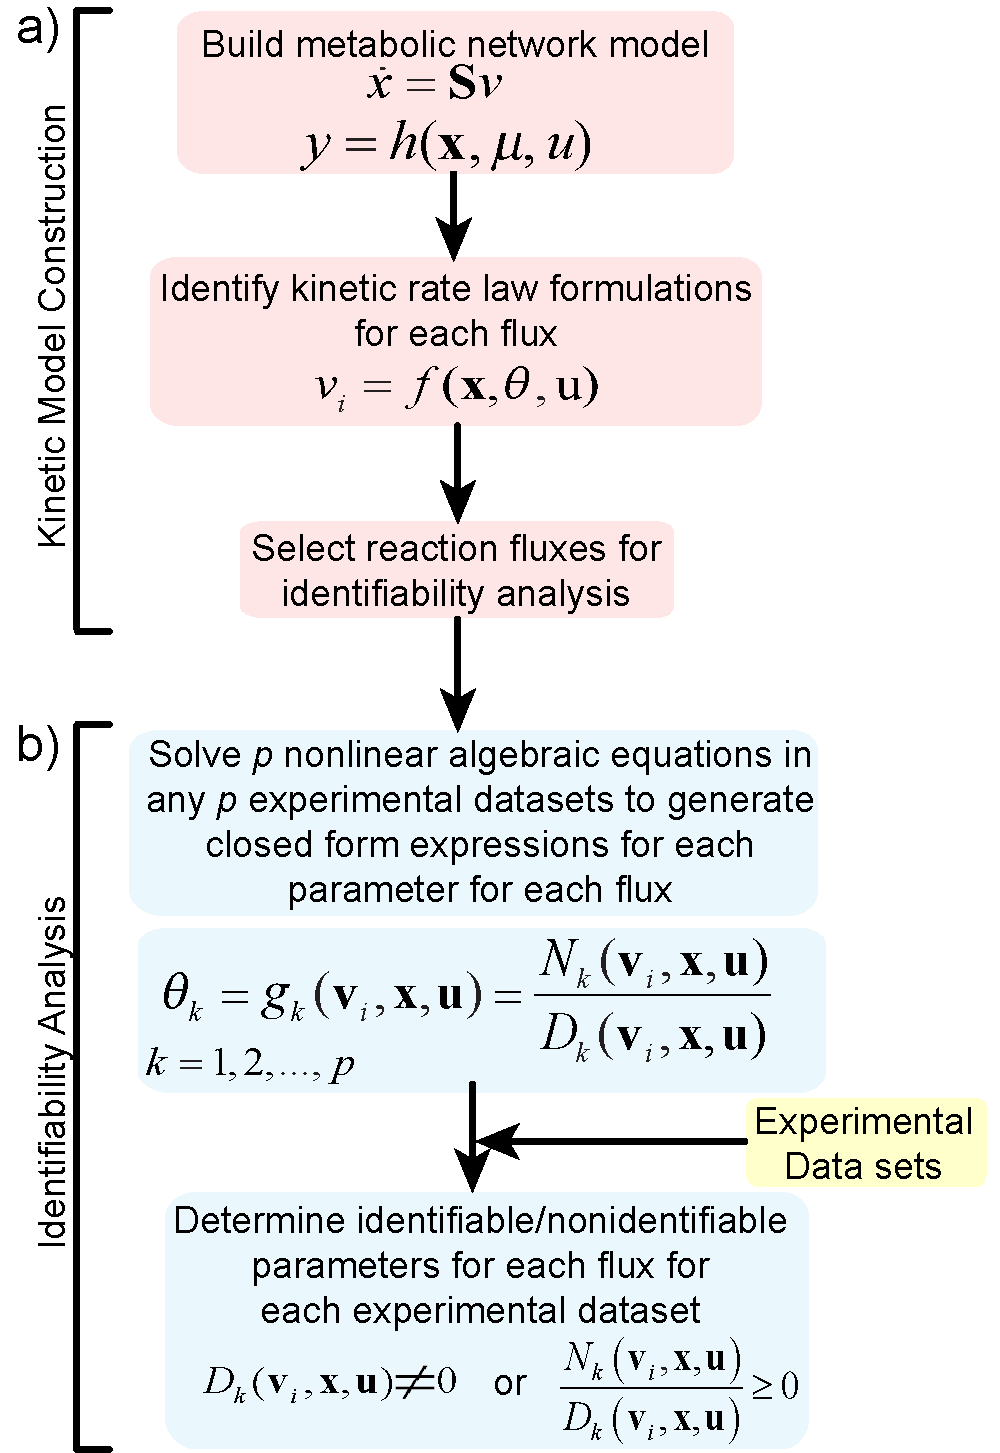
\includegraphics[width=.9\textwidth,height=.6\textheight,keepaspectratio]{figures/figure3/ident_analysis}}
		\caption{A flow diagram showing the methodology developed to establish practical identifiability of parameters in kinetic models of metabolism. a) The steps for the construction of a kinetic model of a metabolic network. The choice of rate law formulations to describe metabolic fluxes influences the identification methodology. The identifiability of parameters for each flux can be established independently. b) The steps for practical identifiability analysis for parameters of a single flux.}\label{fig:ident-flowchart}
	\end{figure}	
	
	\begin{figure}[!tbhp]
		\centering{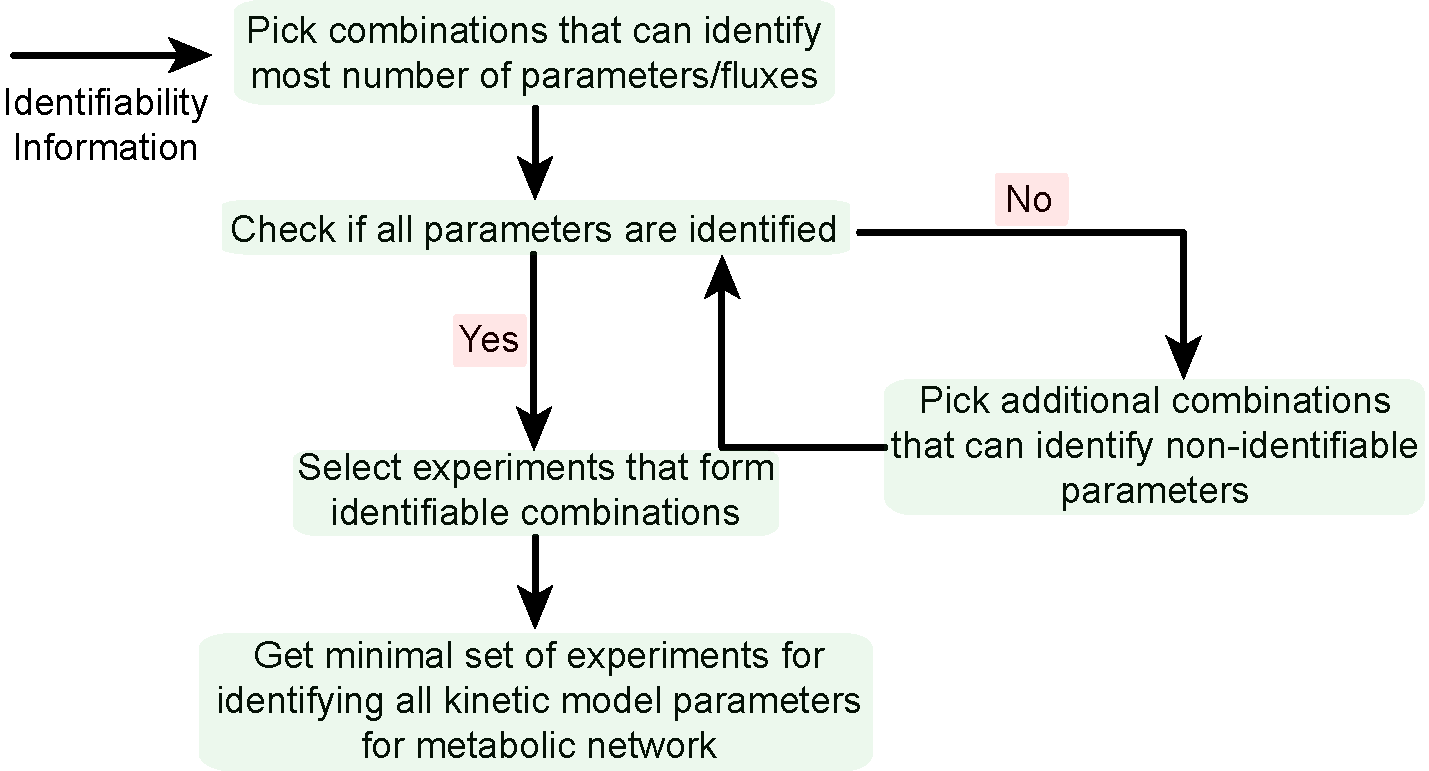
\includegraphics[width=1.0\textwidth,height=1.0\textheight,keepaspectratio]{figures/figure3/experimental_design}}
		\caption{Flow diagram showing a method for experimental design that uses our methodology for practical identification of parameters to determine the number and type of experiments required to identify all fluxes within a given metabolic network.}\label{fig:ident-design}
	\end{figure}

	\begin{figure}[!tbhp]
		\centering{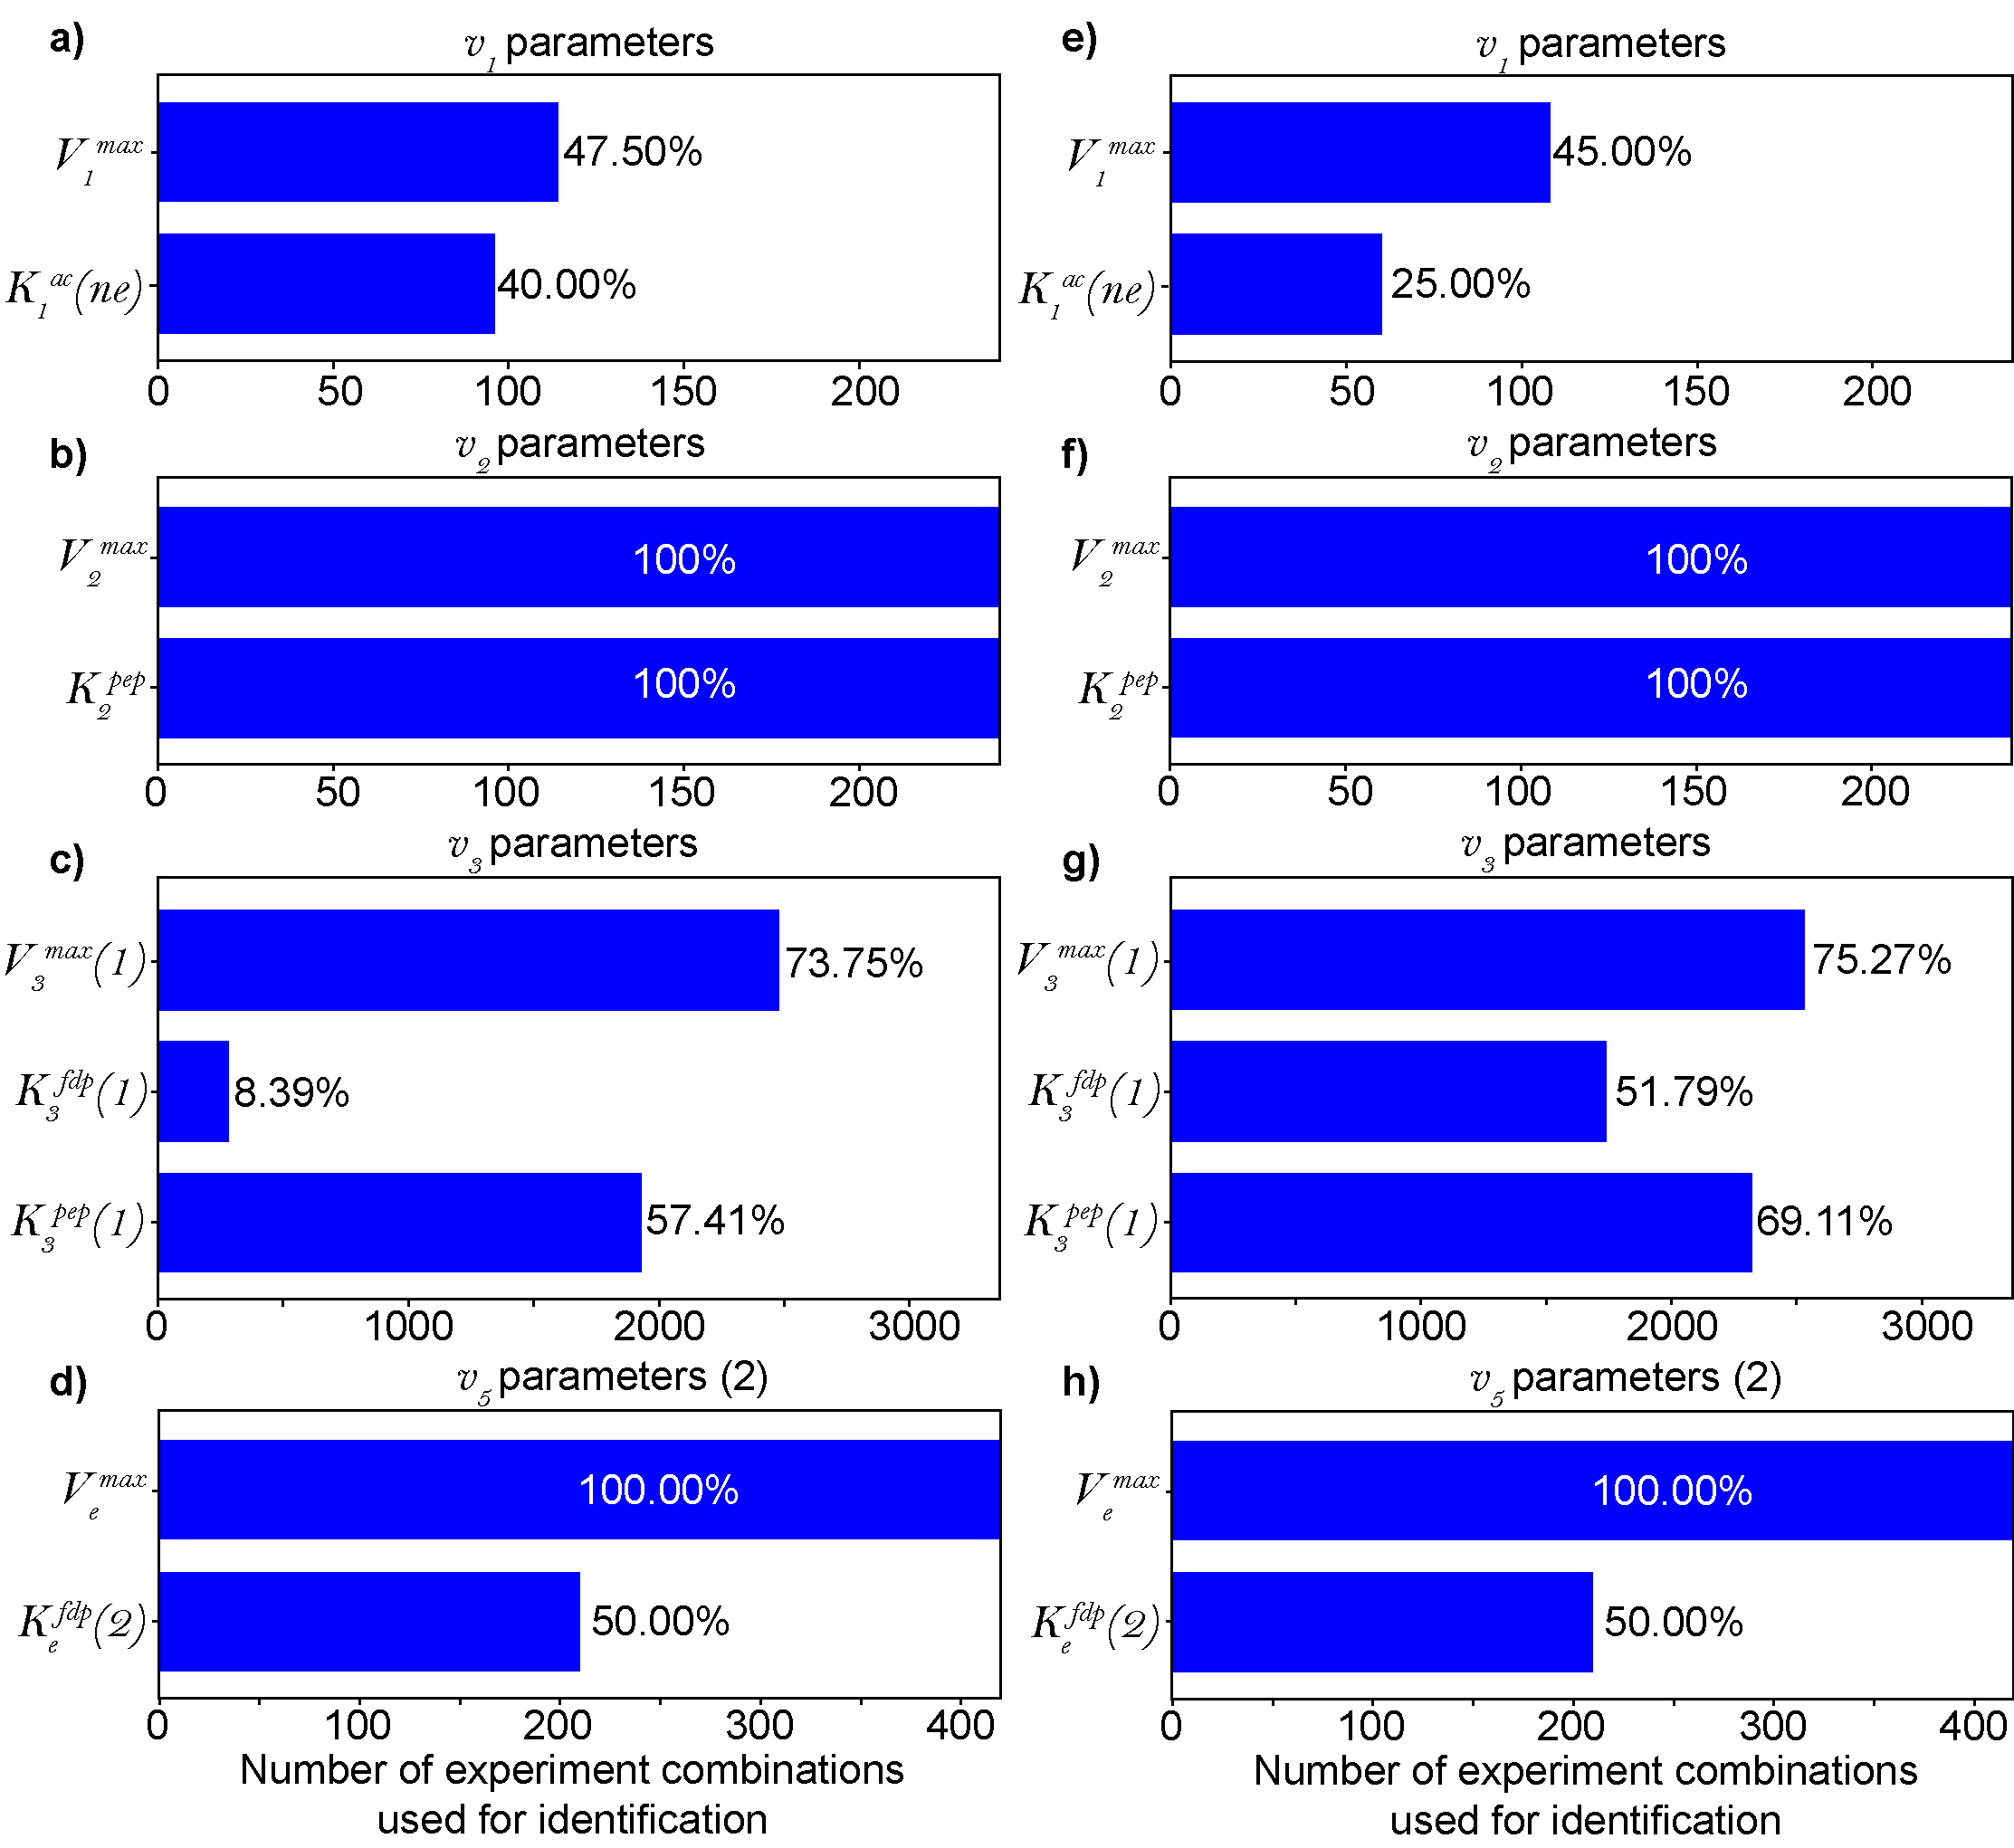
\includegraphics[width=1.0\textwidth,height=0.7\textheight,keepaspectratio]{figures/figure1/v1_V1max_v2_v3_1_v5_mwc_ck_ident}}
		\caption{The number of data combination from 21 different in silico experiments that can practically identify each parameter in fluxes a) and e) $v_1$, b)  and f) $v_2$, c) and g) $v_3$, and d) and h) $v_5$ when there is no noise in the input experimental data. The percentage of total combinations of experimental data used for analysis (240 for $v_1$ and $v_2$, 3360 for $v_3$ and 421 for $v_5$) that can identify each parameter is also specified. $v_1$, $v_2$ and $v_5$ require data from two experiments for analysis, and $v_3$ requires data from three experiments. Results for only one of the two possible roots are shown for $v_3$ and $K_e^{fdp}$ in $v_5$. The results obtained using data from the MWC model for $v_3$ are presented in the panels on the left hand side column and the panels on the right hand column show results obtained using data derived from the Convenience kinetics model for $v_3$.}\label{fig:ident}
	\end{figure}

	\begin{figure}[!tbhp]
		\centering{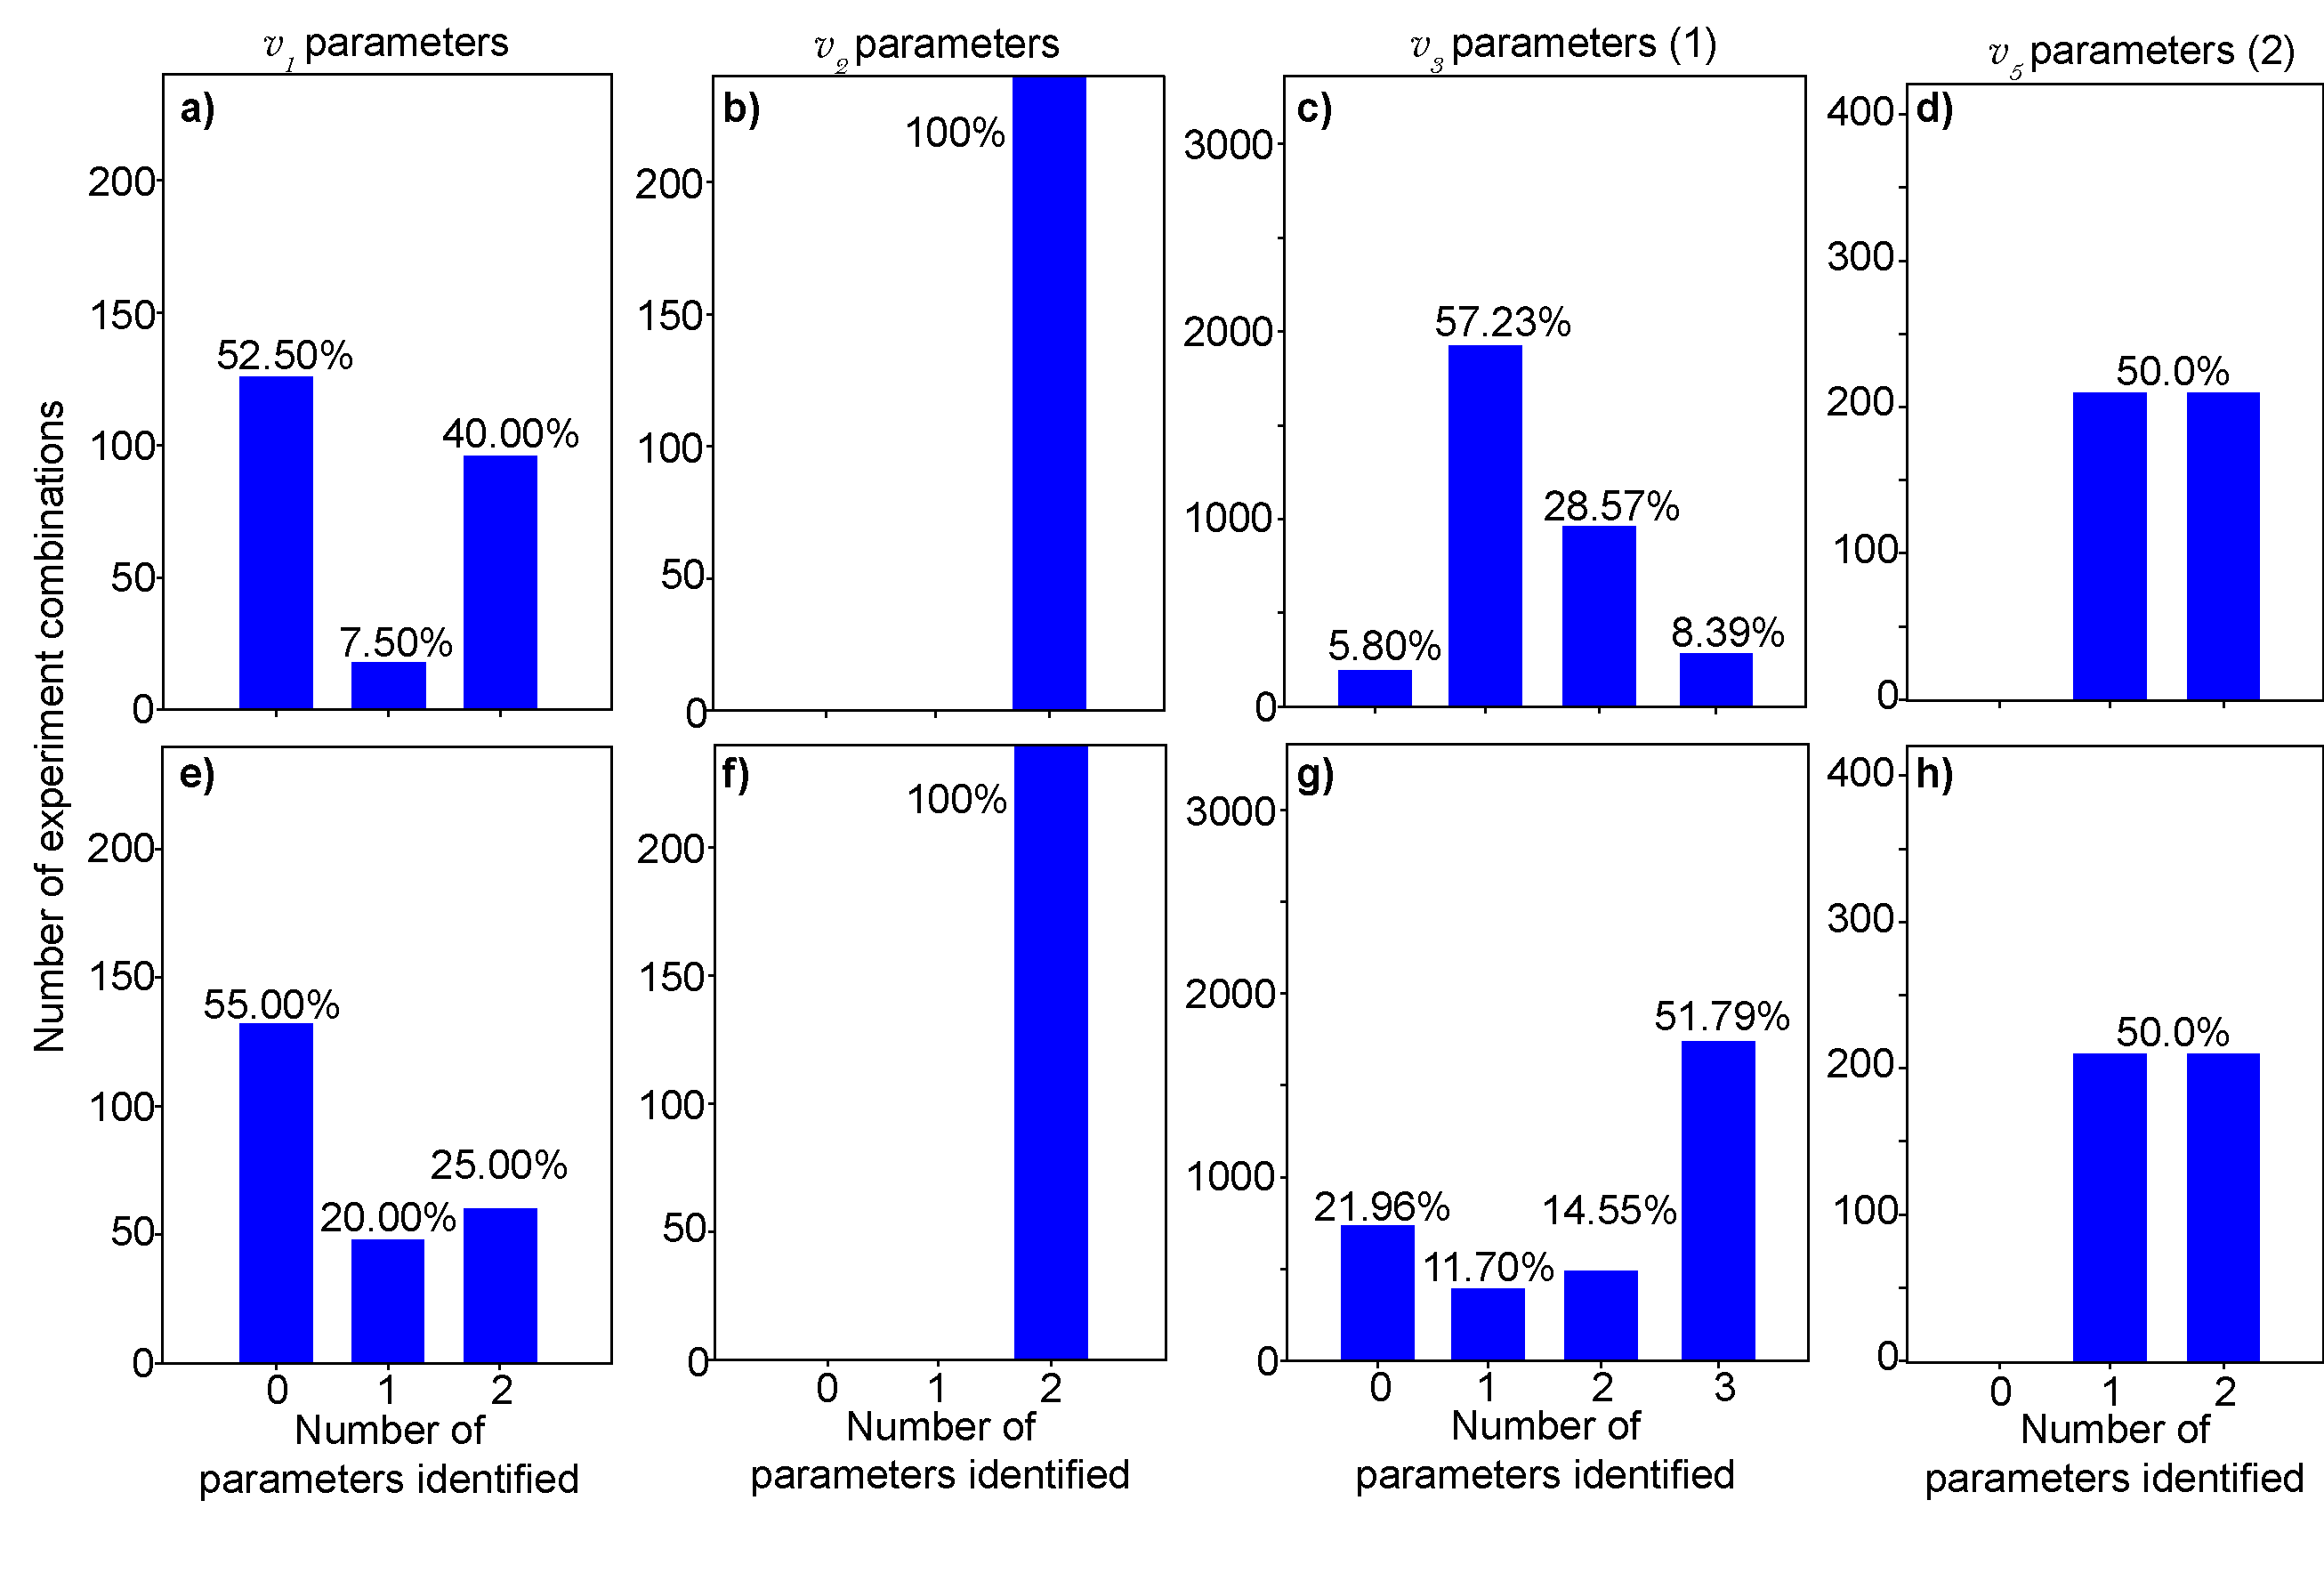
\includegraphics[width=1.0\textwidth,height=0.5\textheight,keepaspectratio]{figures/figure4/v1_V1max_v2_v3_1_v5_2_mwc_ck_data_utility}}
		\caption{Utility of experimental data combinations on the basis of their ability to identify the most number of parameters. Information is shown for parameters modeling fluxes a) $v_1$, b) $v_2$, c) $v_3$ and d) $v_5$. The total number of combinations of experimental data is shown in the vertical axis and the horizontal axis shows the total possible number of parameters that can be identified by data from combinations of a) two, b) two, c) three and d) two experiments. The percentages shown in the plots represent the fraction of the total combinations used to test identifiability of parameters for a given flux. A total of 240 data combinations are used for identifiability analysis for a) $v_1$ and b) $v_2$, 3360 combinations are used to practically identify c) $v_3$, and 420 combinations are used to analyze the identifiability of d) $v_5$. Section \ref{sec:experiments} provides more details on how the combinations of experimental data are generated.}\label{fig:data_utility}
	\end{figure}	

	\begin{figure}[!tbhp]
		\centering{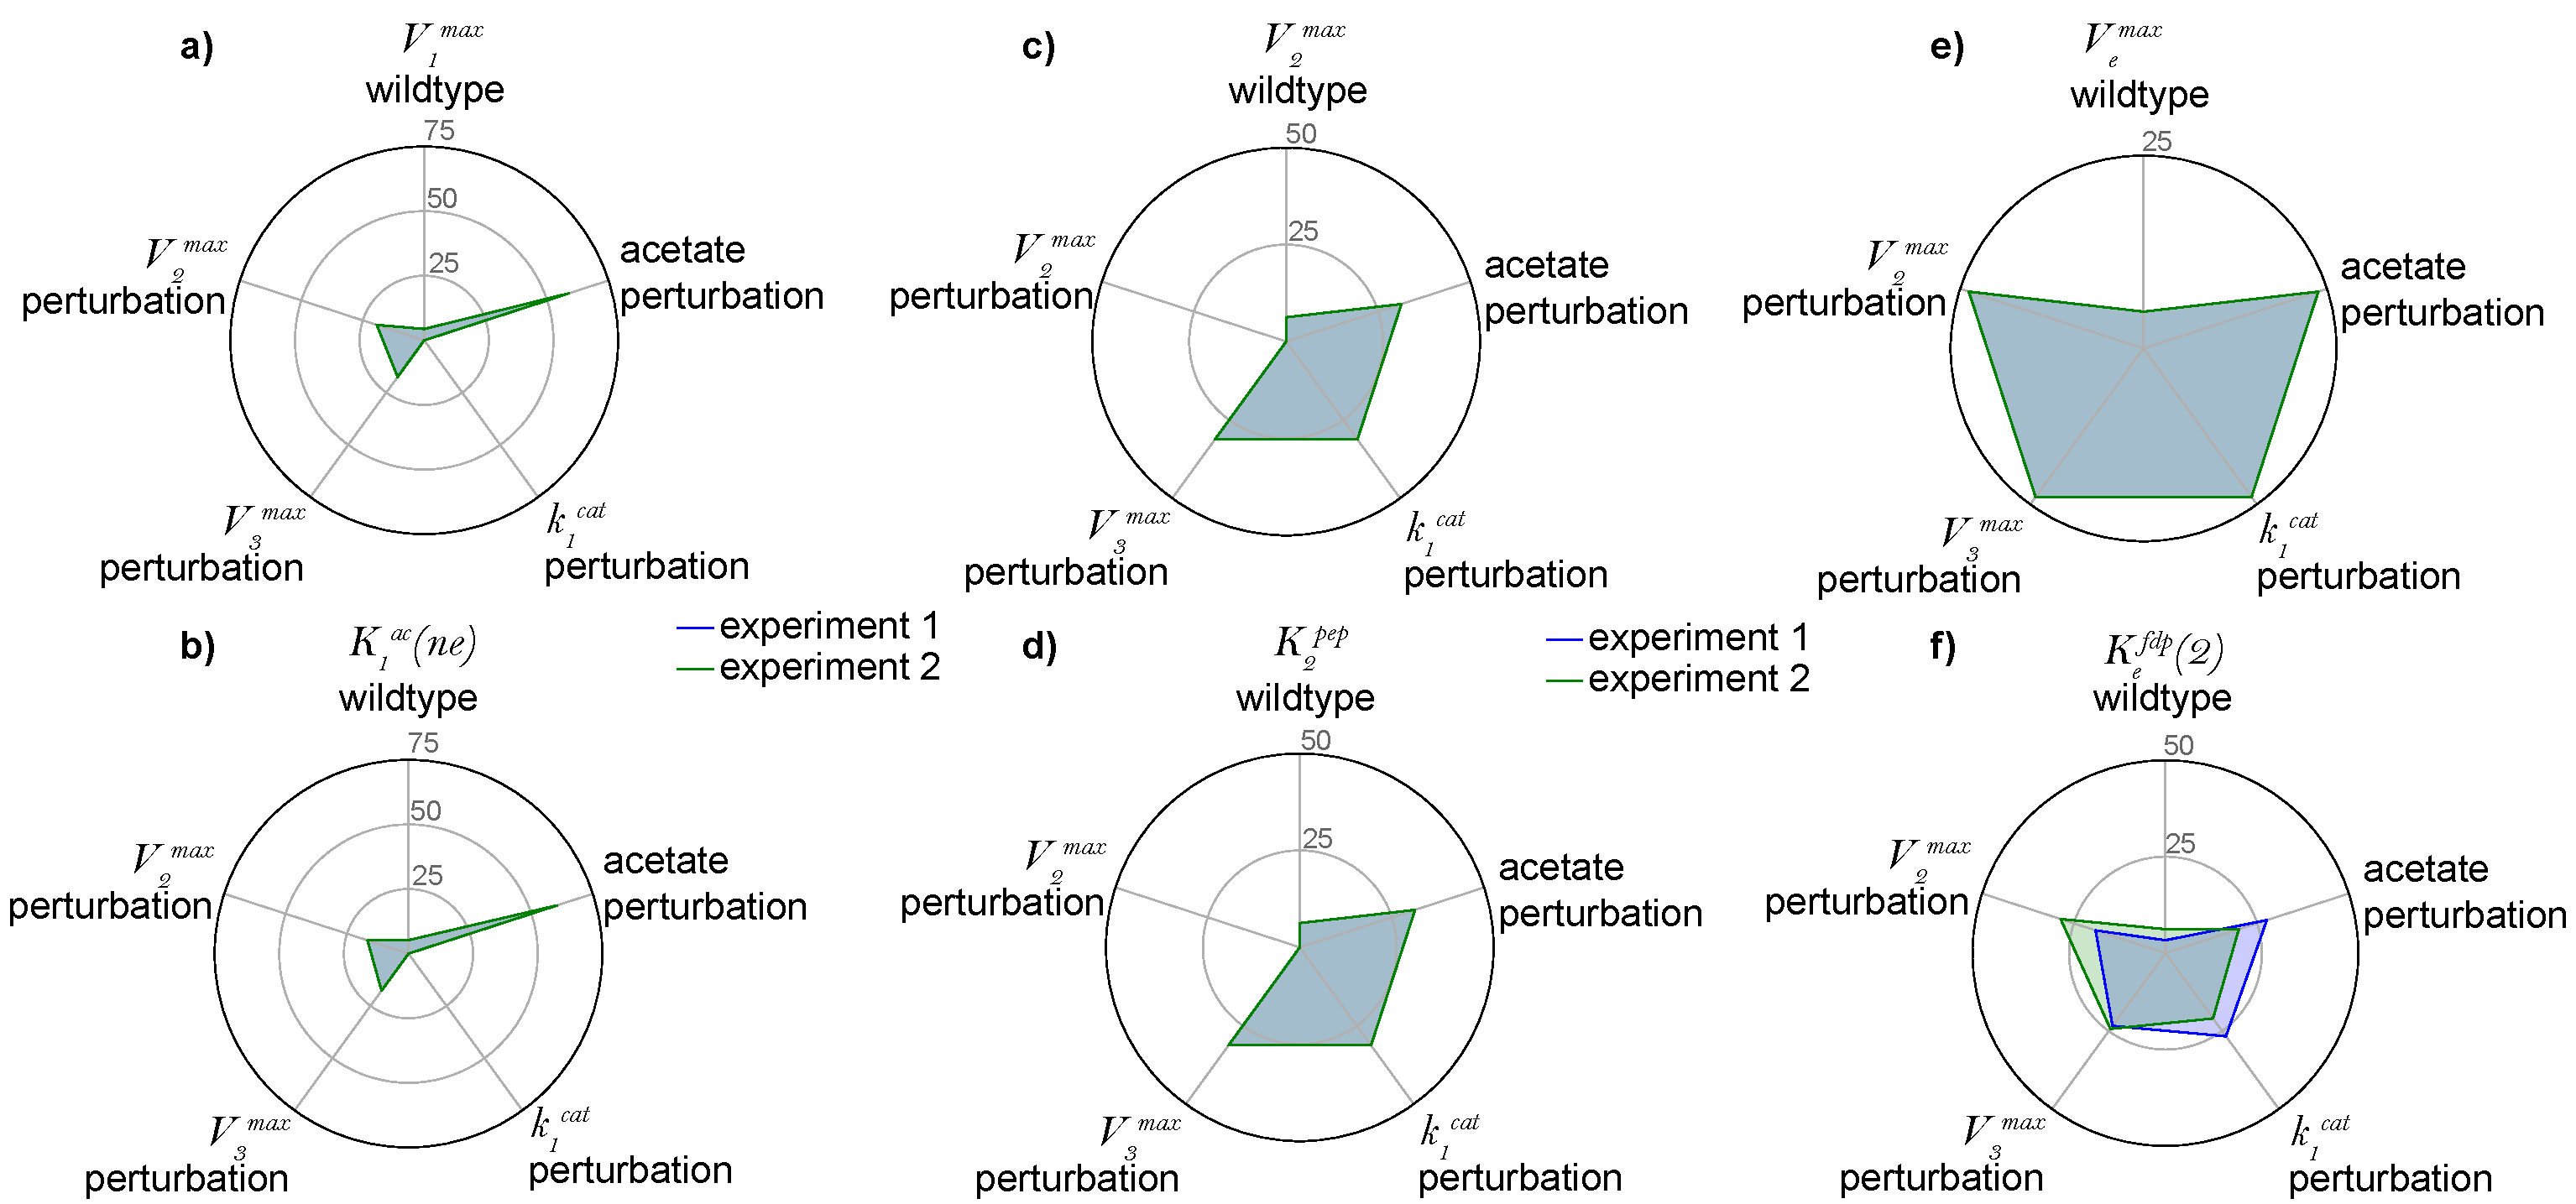
\includegraphics[width=1.0\textwidth,height=0.6\textheight, keepaspectratio]{figures/figure2/v1_V1max_v2_v5_2_exp_info}}
		\caption{The contribution of different experiments types used in a combination of two experiments ($j = \{1, 2\}$) that can practically identify parameter a) $V_1^{max}$, b) $K_1^{ac}$, c) $V_2^{max}$, d) $K_2^{pep}$, e) $V_e^{max}$ and f) $K_e^{fdp}(2)$. The percentages reflect the fractional contribution of each experiment type towards all identifiable data combinations.}\label{fig:exp_info}
	\end{figure} 
	
	\clearpage	

	\section{Old Figures, Figure Captions and other miscellaneous text}	
	Methods and tools for structural identification of parameters based on differential algebra \parencite{Ljung1994, Audoly2001, Bellu2007} and profile likelihood \parencite{Raue2014} are available. However, only the profile likelihood-based methods enable experimental design by facilitating practical identification of parameters. Nonetheless, this method still depend on solving a non-convex nonlinear least squares problem (Equation \ref{eq:lsqopt}) to get likelihood estimates of parameters, and hence still suffers from all the inherent difficulties associated with obtaining global optimal solutions for non-convex optimization problems. This also makes it un-scalable for experimental design and practical identifiability of parameters in kinetic models of large metabolic networks.	
	
\end{document}